\subsection{Overview}
The BBP system is based on a client-server architecture intended to guarantee a separation of responsibilities. The overall structure follows the three-tier architecture pattern, which divides the system into the following logical layers: presentation, application, and data. \\
In general, the system works as follows: the user interacts with the system through either a responsive web application or a native mobile app. These interfaces send requests via secure HTTPS protocol and RESTful APIs to a central server. The server verifies the user's identity, processes requests by applying business rules, and coordinates interaction with third-party services for geographic and meteorological features. Finally, persistent data is saved and retrieved by a database management system optimized for spatial data. \\
The components that make up these levels are described in detail below:

\subsubsection{Presentation Layer}
The presentation layer consists of two components:
\begin{itemize}
    \item \textbf{Web Application}: A Single Page Application developed with the Vue.js framework. This component resides on the user's device and provides a dynamic user experience. Its main functions include managing the user interface by rendering pages and forms for registration and login, as well as geographical visualization through the integration of interactive maps to show routes and obstacles.
    \item \textbf{Mobile Application}: A native mobile app developed with Flutter framework that includes all web functionalities plus real-time GPS tracking for both trip recording and bike path creation, with automatic obstacle detection via device sensors (accelerometer, gyroscope).
\end{itemize}

\subsubsection{Application Layer}
The backend is a server application based on Java Spring Boot. This layer exposes a set of RESTful APIs that serve as a single point of entry for the presentation layer. One of the most critical parts of the project is the security of the user's personal data, therefore it is in the application layer where most of the security resides, access to private accounts is implemented through credential verification and JSON Web Tokens validation for each request. The server processes users' data by implementing domain logic, such as calculating travel statistics and validating the quality of bike routes. Finally, it also handles the API requests to external services (Mapbox for routing/geocoding, Open-Meteo for weather data) and transforms raw data into useful information for the user.

\subsubsection{Data Layer}
Persistence is handled by the relational database PostgreSQL. A key feature of this layer is the use of the spatial extension PostGIS. The database stores both simple types such as integers and strings but also complex geometries; this allows the system to perform efficient spatial queries directly at the database level.

\subsubsection{External Services}
The BBP system uses external services for functions that are too complex to be made for this project. Specifically, Mapbox is used for both the geocoding service, that means converting addresses into coordinates, and the routing engine needed to calculate the best route. BBP also uses Open-Meteo to enrich travel data with historical weather information based on date and location.

\subsubsection{Architectural Diagrams}
To visualize the structure described above, the architectural diagram of the system is shown below. Figure \ref{fig:high_level_arch} illustrates the high-level architecture, showing the communication flows between the clients, server, database, and external services.

\begin{figure}[H]
    \centering
        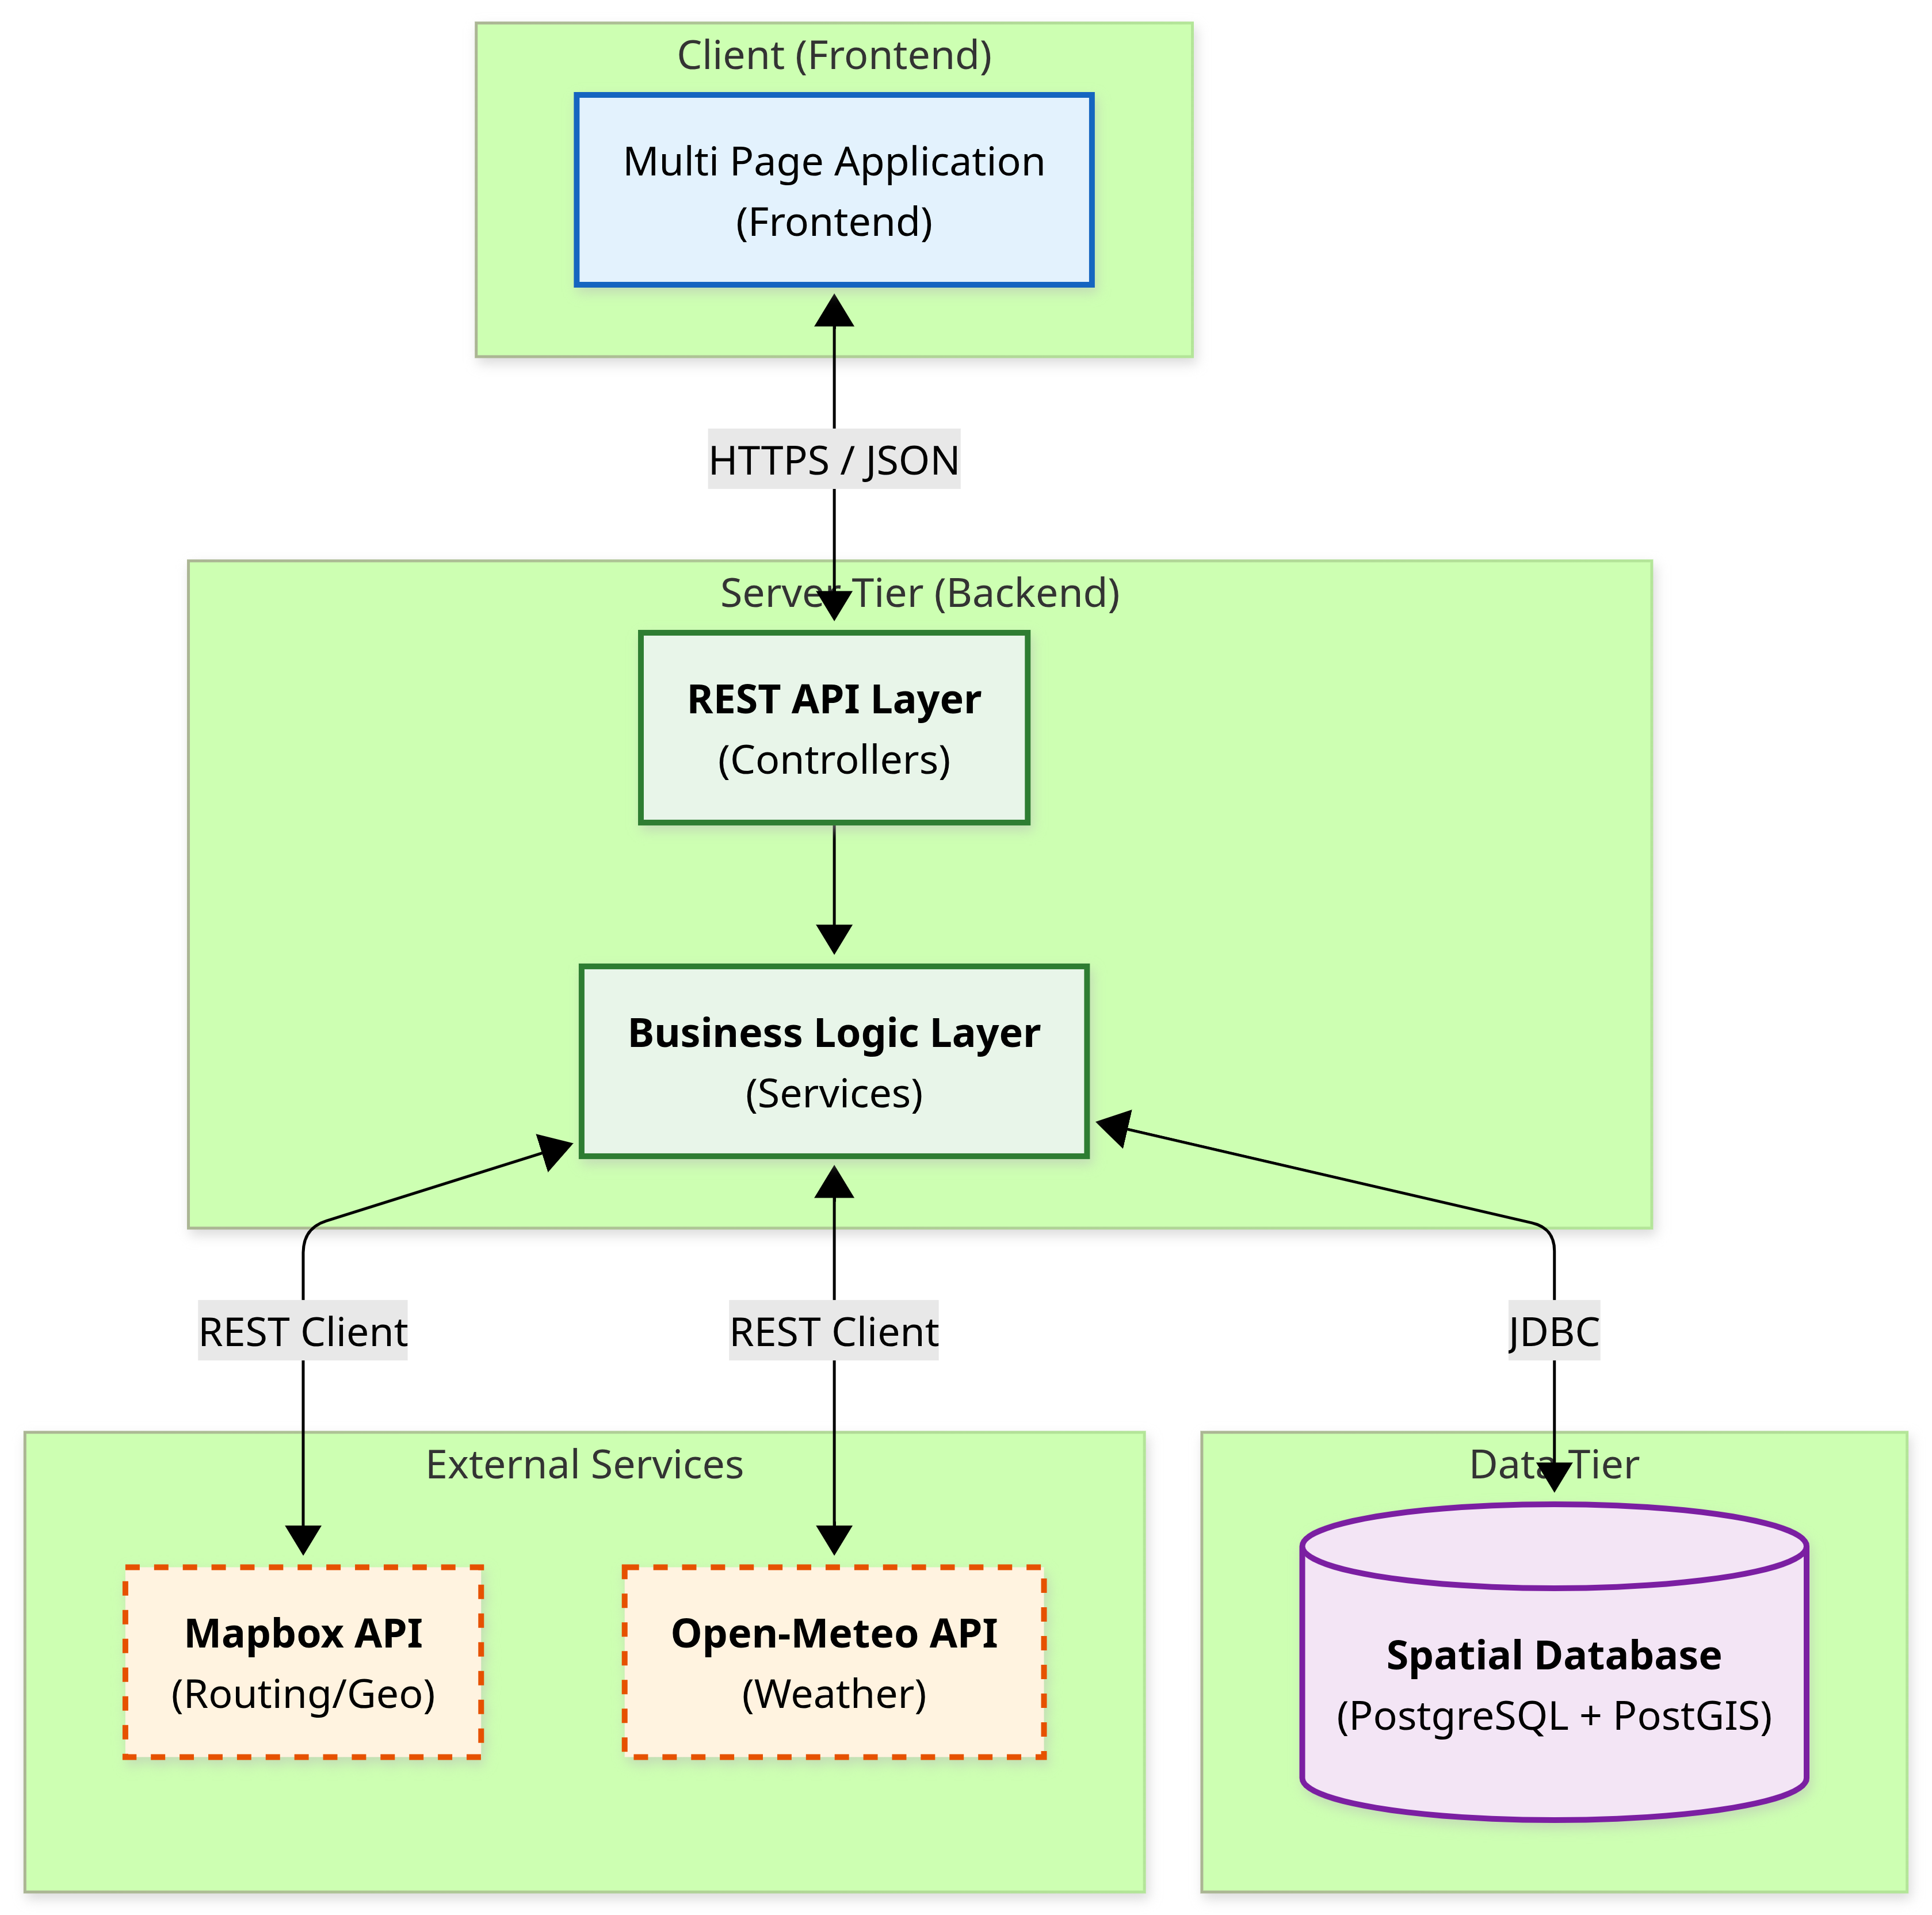
\includegraphics[width=\linewidth, height=\textheight, keepaspectratio]{DD/images/high-level-arch.png}
    \caption{High level architecture of the system}
    \label{fig:high_level_arch}
\end{figure}

\subsection{Component View}
The BBP system consists of several software components that work together to provide the functionality described in the RASD. The architecture, as stated previously, is based on the client-server paradigm, with a distinct separation between business logic, also known as backend, the user interface, also known as frontend, and the external services.

\subsubsection{Backend Components}
The backend is a monolithic application managed by the Spring Boot framework; each service is responsible for a distinct functional domain and exposed via REST API.

\begin{itemize}
    \item \textbf{Authentication Service}: This component manages the security and access on the platform; it's implemented with UserAuthService and JwtService, and it handles the processes of registration, login, and the generation of JSON Web Token.
    
    \item \textbf{User Management Service}: This component manages the user profile. It allows users to modify their credentials and manage their personal data.
    
    \item \textbf{Trip Service}: This component manages the trip recording and history. It saves all necessary data collected during biking sessions and calculates statistics. It also performs data enrichment as, at the end of a trip, the service makes a request to the external Weather Data Provider to associate historical weather conditions with the time and location of the completed activity.
    
    \item \textbf{Obstacle Management Service}: This component is responsible for the handling of the obstacles, it receives the obstacles reports, both manually inserted and automatically detected, it then validates that the obstacles are within a buffer distance from the bike path, and if so, it saves them in the database and triggers the recalculation of the path's quality score.

    \item \textbf{Sensor Analysis Service}: This component is responsible for the validation and enrichment of the anomalies detected by the mobile app. It receives preliminary obstacle detections with their location and context, then uses algorithms to calculate a confidence score based on pattern analysis. Additionally, it performs cross-validation by checking if other users have reported obstacles in the same geographical area. In the end it enriches the anomalies with confidence scores and cross-validation data, then sends the results back to the mobile app for user confirmation.
    
    \item \textbf{Bike Path Service}: This component manages the creation and modification of bike paths. It implements the logic to compute the Quality Score based on the road surface conditions and the total number of obstacles associated with the path.
    
    \item \textbf{Bike Path Finder Service}: This component processes the spatial queries for locating the routes within a geographical area and it applies the filter specified by the user.
    
    \item \textbf{Mapbox Integration Service}: This component acts as a wrapper for Mapbox APIs, it decouples the backend from the external service provider, it handles the geocoding and the provision of the tokens required for client-side rendering.

    \item \textbf{Open-Meteo Integration Service}: This component acts as a wrapper for Open-Meteo APIs, it decouples the backend from the external weather data provider, it handles the retrieval of historical weather data based on location and time.
\end{itemize}

\subsubsection{Frontend Components}
\begin{itemize}
    \item \textbf{Web Application}: This component represents the main point of interaction for users via web browser. It is a Single Page Application developed with Vue.js that communicates with the backend via REST API. It manages the display of dashboards, interactive maps, and user profiles.
    
    \item \textbf{Mobile Application}: This component provides all web functionalities plus real-time GPS tracking and automatic obstacle detection. It interfaces with the device hardware to collect data from GPS, accelerometer, and gyroscope, processes sensor data locally to detect preliminary anomalies, and sends them to the backend for validation and enrichment. After receiving confidence scores and cross-validation data from the server, it requests user validation before sending the final obstacle reports to the backend.
\end{itemize}

\subsubsection{Data Layer}
\begin{itemize}
    \item \textbf{DBMS}: This component acts as central storage for all system data, it uses a relational database with a spatial extension to handle geolocated entities such as bike paths, trips, and obstacles.
\end{itemize}

\subsubsection{External Services}
These components are external to the BBP system but essential for its operation.
\begin{itemize}
    \item \textbf{Map Provider (Mapbox)}: This component provides the mapping functionalities, such as interactive map tiles and accurate routing data.
    
    \item \textbf{Weather Data Provider (Open-Meteo)}: This component provides historical and current weather data.
\end{itemize}

\begin{figure}[H]
    \centering
        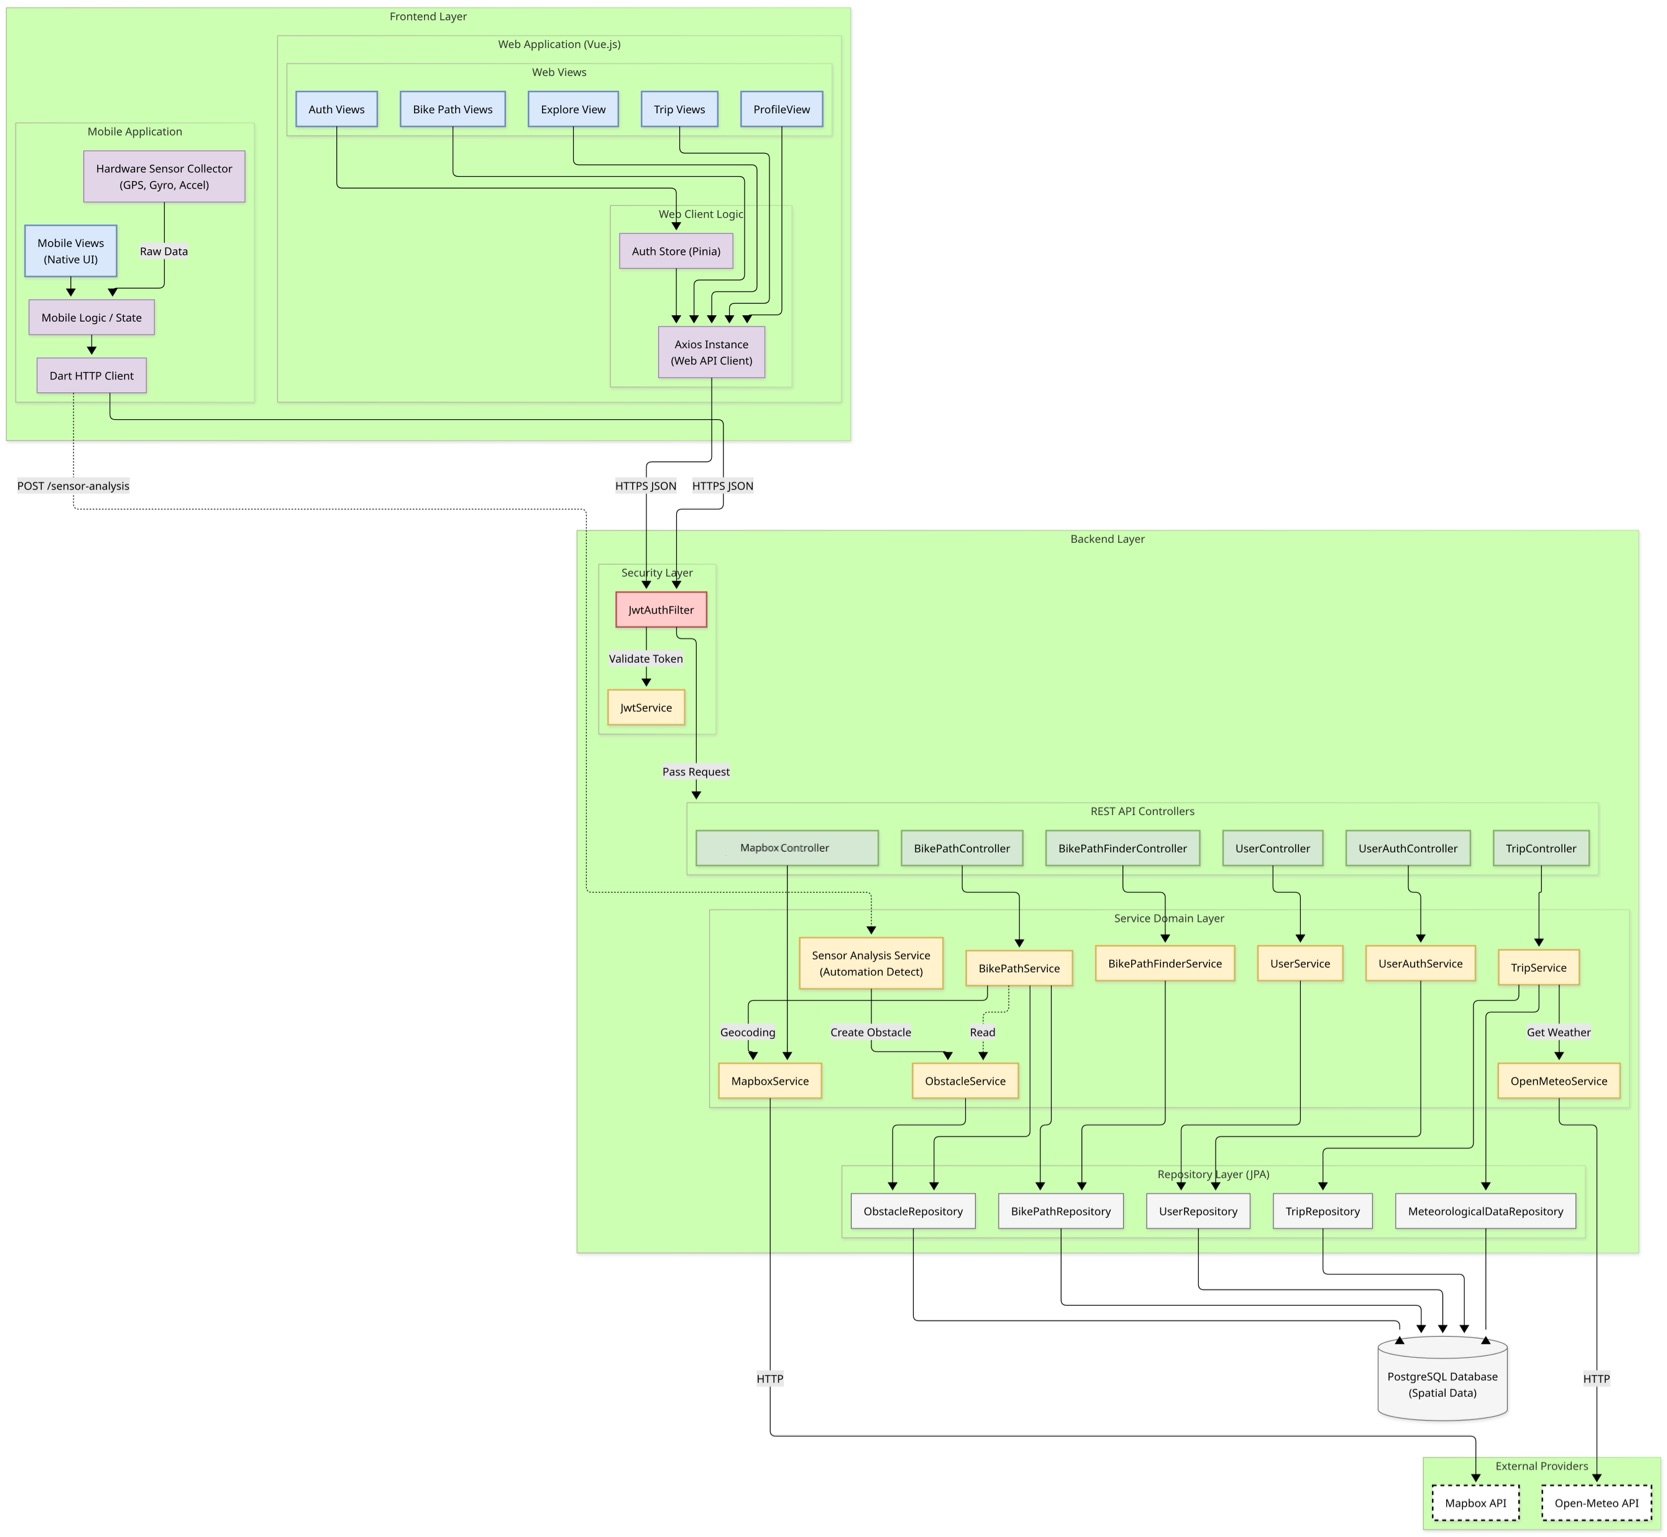
\includegraphics[width=\linewidth, height=\textheight, keepaspectratio]{DD/images/component-view.jpg}
    \caption{Component view}
    \label{fig:component-view}
\end{figure}

\clearpage

\subsection{Deployment View}
BBP system adopts a distributed architecture based on the three-tier model; its software components reside on physically separated nodes and interact with each other via standard network protocols.

\subsubsection{Nodes Deployment}

\begin{itemize}
    \item \textbf{Client Node}: This node identifies the user's device; the execution environment requires a modern web browser that supports HTML5 and JavaScript in the case the user uses the web interface, otherwise it needs a phone with the most recent Android or iOS version. Moreover, for the automatic detection to work, the client node will need a gyroscope and an accelerometer.

    \item \textbf{Web Server}: This node is hosted on the cloud and uses a reverse proxy to handle requests on port 443. It distributes the static files of the frontend and acts as a gateway by forwarding the API calls to the Application Server.
    
    \item \textbf{Application Server}: This node constitutes the core of the backend infrastructure and is hosted on the cloud. The execution environment launches the Java artifact, where the Spring Boot application incorporates a Tomcat server listening on port 8080.

    \item \textbf{Database Server}: This node runs on a dedicated server for data persistence, the DBMS is PostgreSQL with the PostGIS extension enabled to provide native support for geospatial data.

    \item \textbf{External Service Providers}: These are third-party systems necessary for the operation of BBP. In particular, Mapbox provides APIs for vector maps, routing, and geocoding, while Open-Meteo provides APIs for retrieving historical and current weather data.
\end{itemize}

\begin{figure}[H]
    \centering
        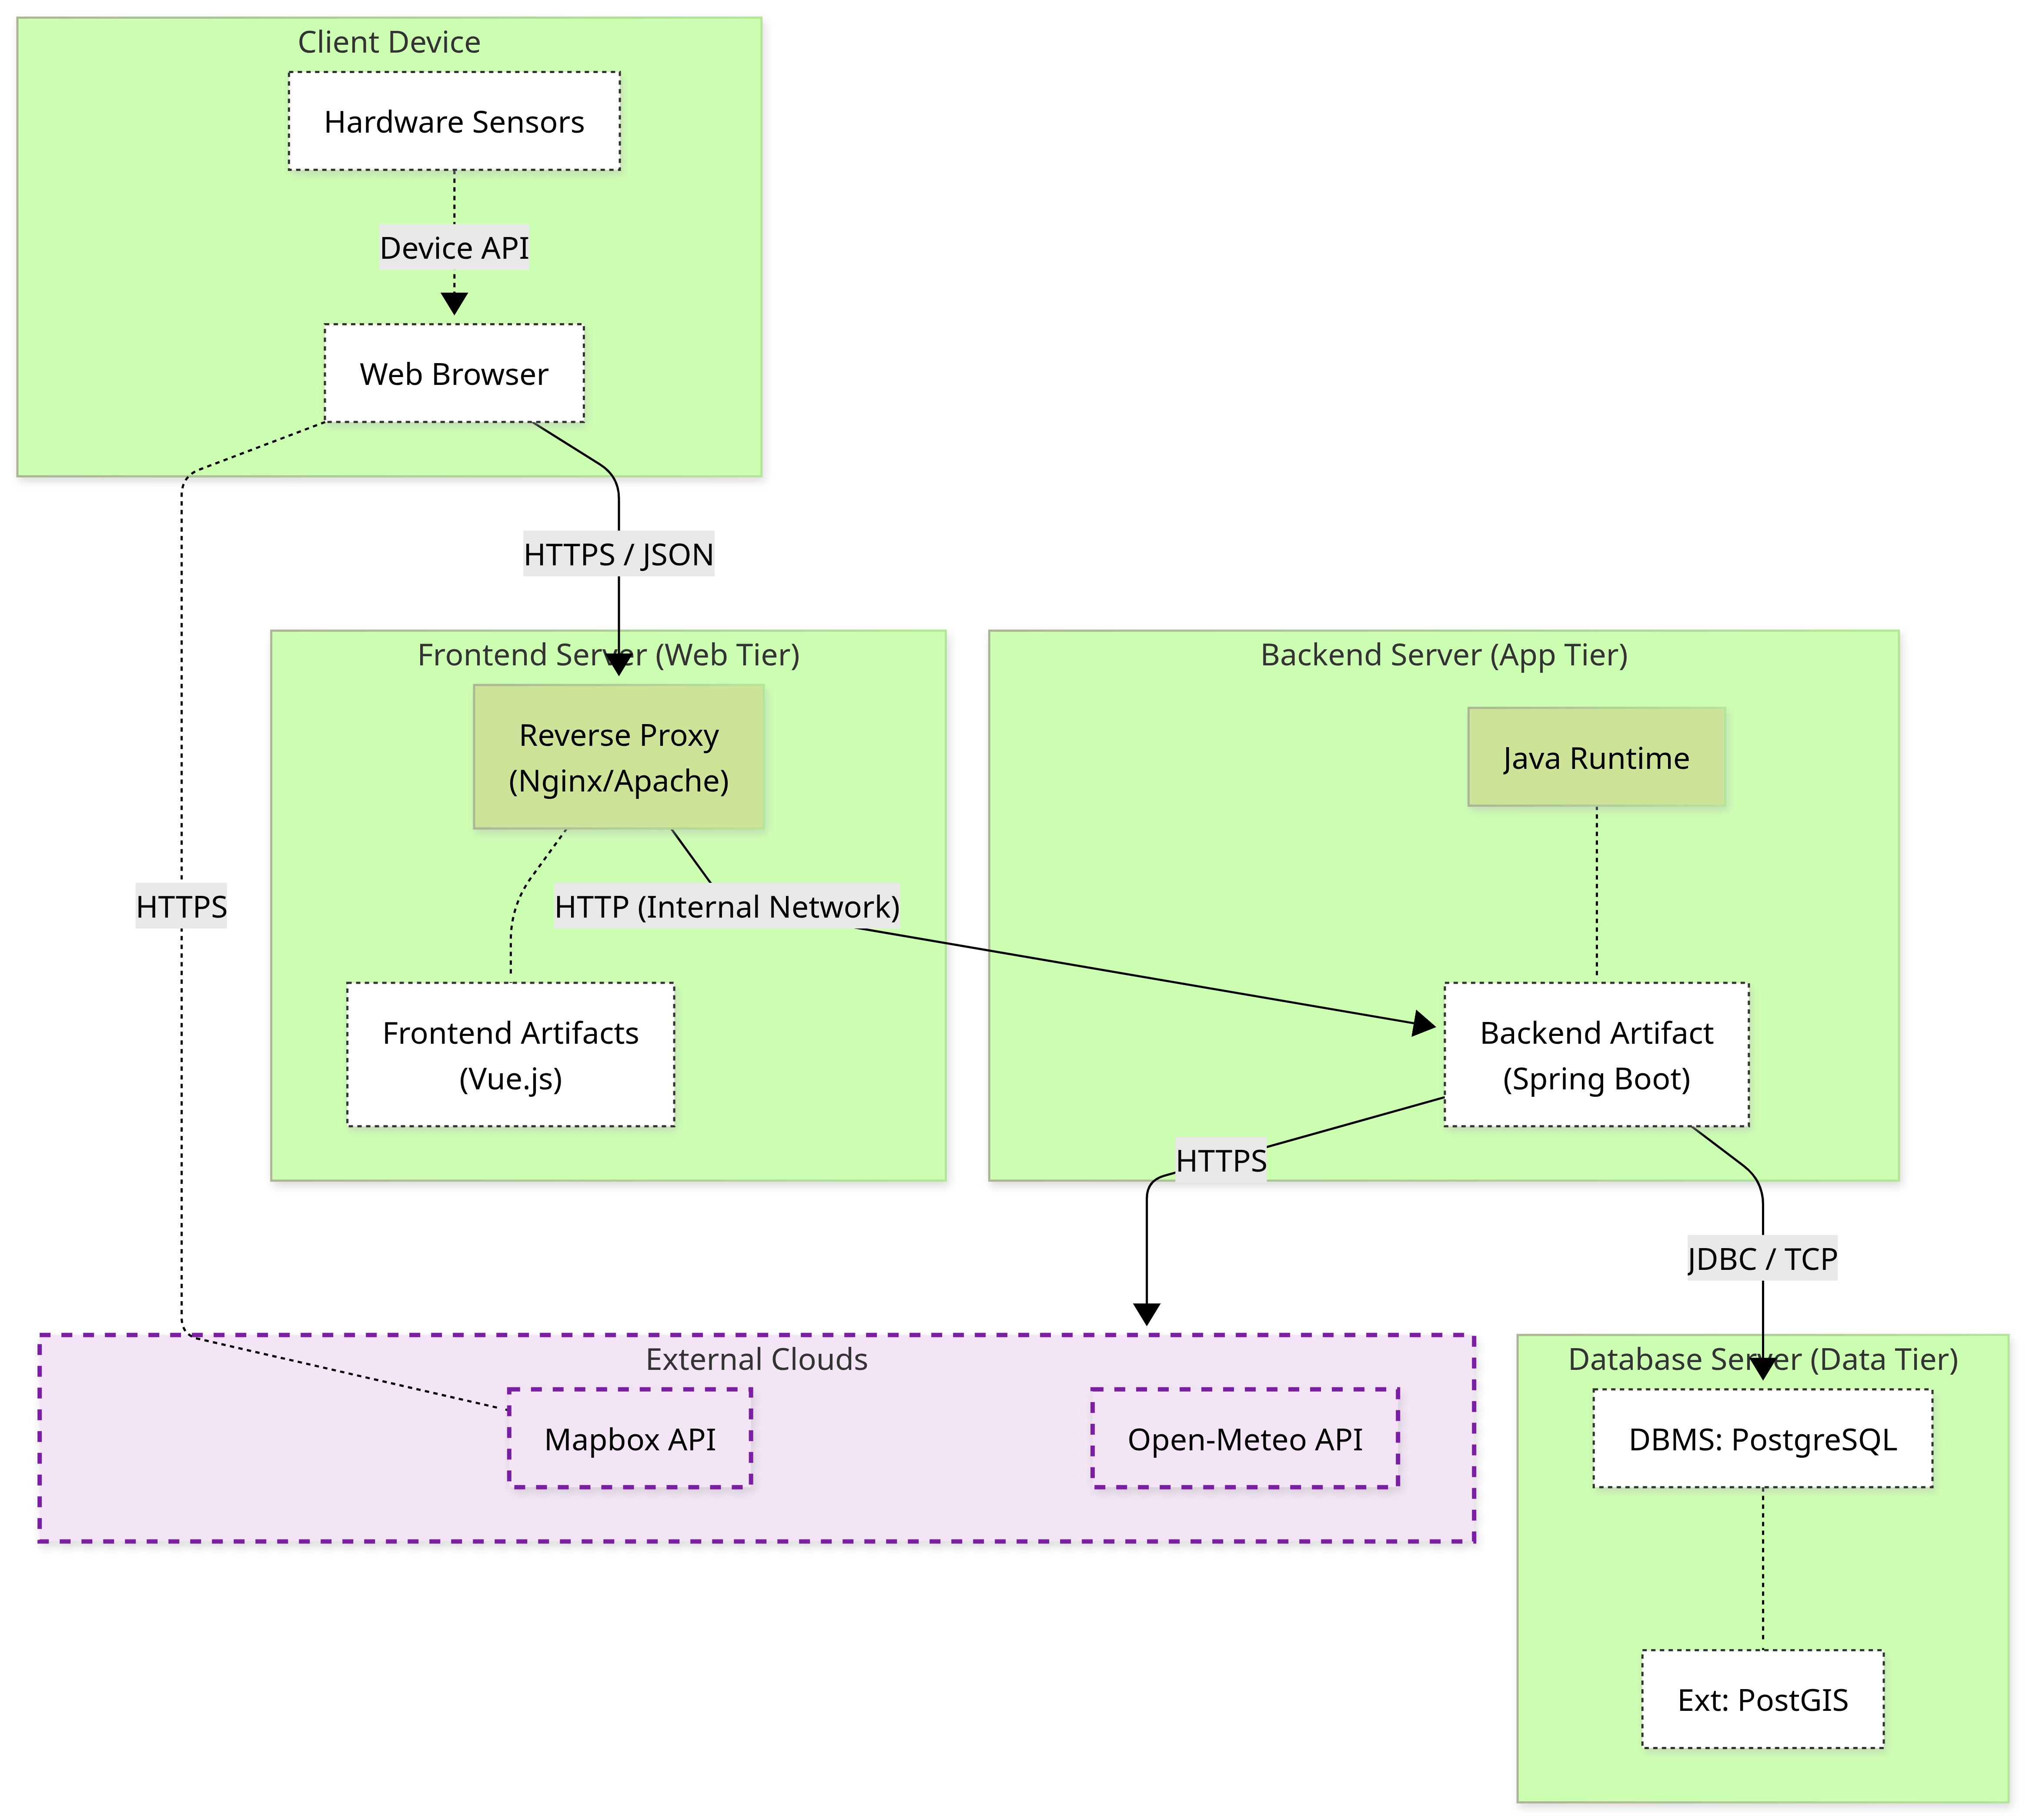
\includegraphics[width=\linewidth, height=\textheight, keepaspectratio]{DD/images/deployment-view.png}
    \caption{Deployment view}
    \label{fig:deployment-view}
\end{figure}
\clearpage

\subsection{Runtime view}
This section describes the dynamic interaction between system components that realize the use cases.

\noindent
\textbf{UC1: Manual Trip Insertion} \\
The user manually inserts a trip specifying the route taken and the timing. After the submission, TripService invokes the MapboxService to calculate the exact geometry of the trip and the travelled distance, then it makes an API request to the Open-Meteo service to get the historical weather conditions at the time of the trip. In the end it saves the entity in the database and sends the user a confirmation.

\begin{figure}[H]
    \centering
        \includegraphics[width=\linewidth, height=\textheight, keepaspectratio]{DD/images/seq_uc1.png}
    \caption{Sequence Diagram - UC1 Manual Trip Insertion}
    \label{fig:seq_uc1}
\end{figure}

\clearpage

\noindent
\textbf{UC2: Creation of a Public Bike Path} \\
The user creates a bike path by defining waypoints on a map. The system receives these waypoints and uses the Mapbox service to calculate the exact path geometry. A spatial validation is performed to ensure that the obstacles are within a buffer distance from the route, then the system calculates the Quality Score and saves the bike path with the visibility settings chosen by the user.

\begin{figure}[H]
    \centering
        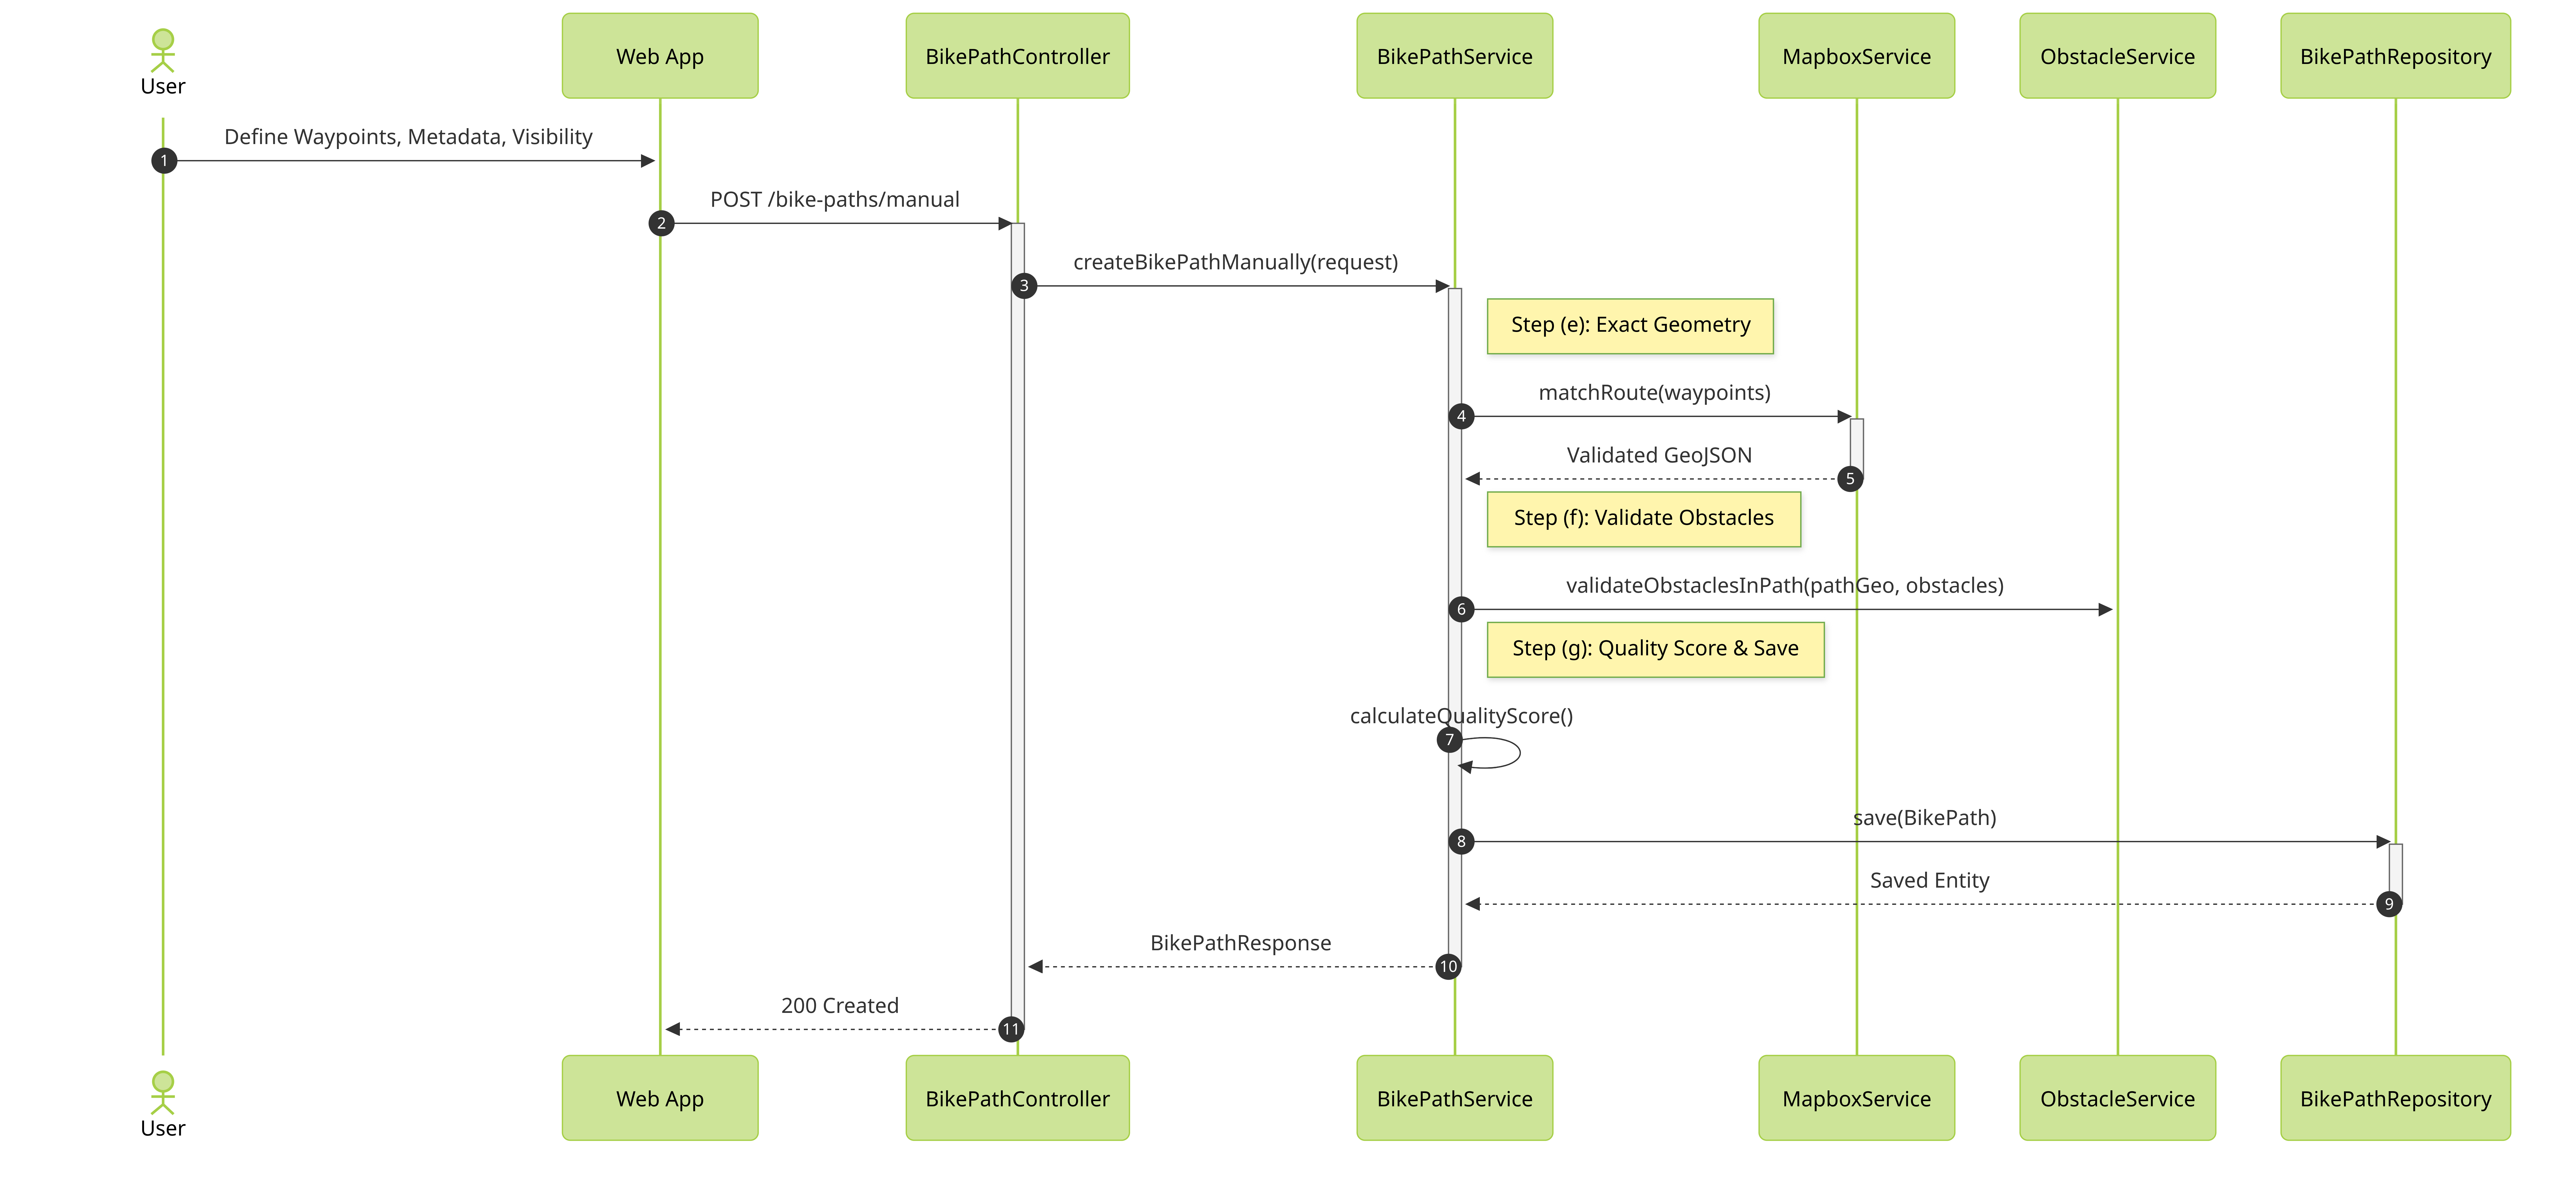
\includegraphics[width=\linewidth, height=\textheight, keepaspectratio]{DD/images/seq_uc2.png}
    \caption{Sequence Diagram - UC2 Creation of a Public Bike Path}
    \label{fig:seq_uc2}
\end{figure}

\clearpage

\noindent
\textbf{UC3: Search of Bike Paths} \\
The user searches for bike paths by entering the origin and destination. The BikePathFinderService geocodes the addresses and performs a spatial query delegated to PostGIS to find published routes in the requested area. The database uses spatial indexes and native PostGIS functions to efficiently filter routes by proximity to both the starting point and destination point, and returns the complete bike path data including route geometry and obstacles. Results are sorted by descending score and displayed to the user.

\begin{figure}[H]
    \centering
        \includegraphics[width=\linewidth, height=\textheight, keepaspectratio]{DD/images/seq_uc3.png}
    \caption{Sequence Diagram - UC3 Search of Bike Paths}
    \label{fig:seq_uc3}
\end{figure}

\clearpage

\noindent
\textbf{UC4: Obstacle Reporting on Bike Path} \\
A user reports an obstacle on an existing bike path. After receiving the report, the system verifies the geographical consistency of the obstacle with respect to the geometry of the bike path. If valid, the obstacle is saved, the Quality Score is recalculated, and the update is made visible to all users.

\begin{figure}[H]
    \centering
        \includegraphics[width=\linewidth, height=\textheight, keepaspectratio]{DD/images/seq_uc4.png}
    \caption{Sequence Diagram - UC4 Obstacle Reporting}
    \label{fig:seq_uc4}
\end{figure}

\clearpage

\noindent
\textbf{UC5: Automatic Bike Path Creation} \\
While the user is cycling, the mobile app records the route and identifies potential obstacles locally with a low degree of confidence using device sensors. When the user stops, the app detects the stop, finalizes the route, and sends preliminary obstacle data to the SensorAnalysisService. The backend enriches the anomalies by calculating confidence scores based on pattern analysis and performing cross-validation by checking if other users have reported obstacles in the same geographical area. The server responds with the enriched obstacle data, and the app then displays a prompt to the user to validate or modify the detected obstacles. After user validation, the app sends the complete payload to the server, which creates the bike path with validated obstacles via the BikePathService.

\begin{figure}[H]
    \centering
        \includegraphics[width=\linewidth, height=\textheight, keepaspectratio]{DD/images/seq_uc5.png}
    \caption{Sequence Diagram - UC5 Automatic Bike Path Creation}
    \label{fig:seq_uc5}
\end{figure}

\clearpage

\noindent
\textbf{UC6: User Registration} \\
The user submits registration data including email and password. The system validates the uniqueness of the email and the correctness of the inserted data. It creates the new account by hashing the password, generates a session token, and redirects the user to the dashboard.

\begin{figure}[H]
    \centering
        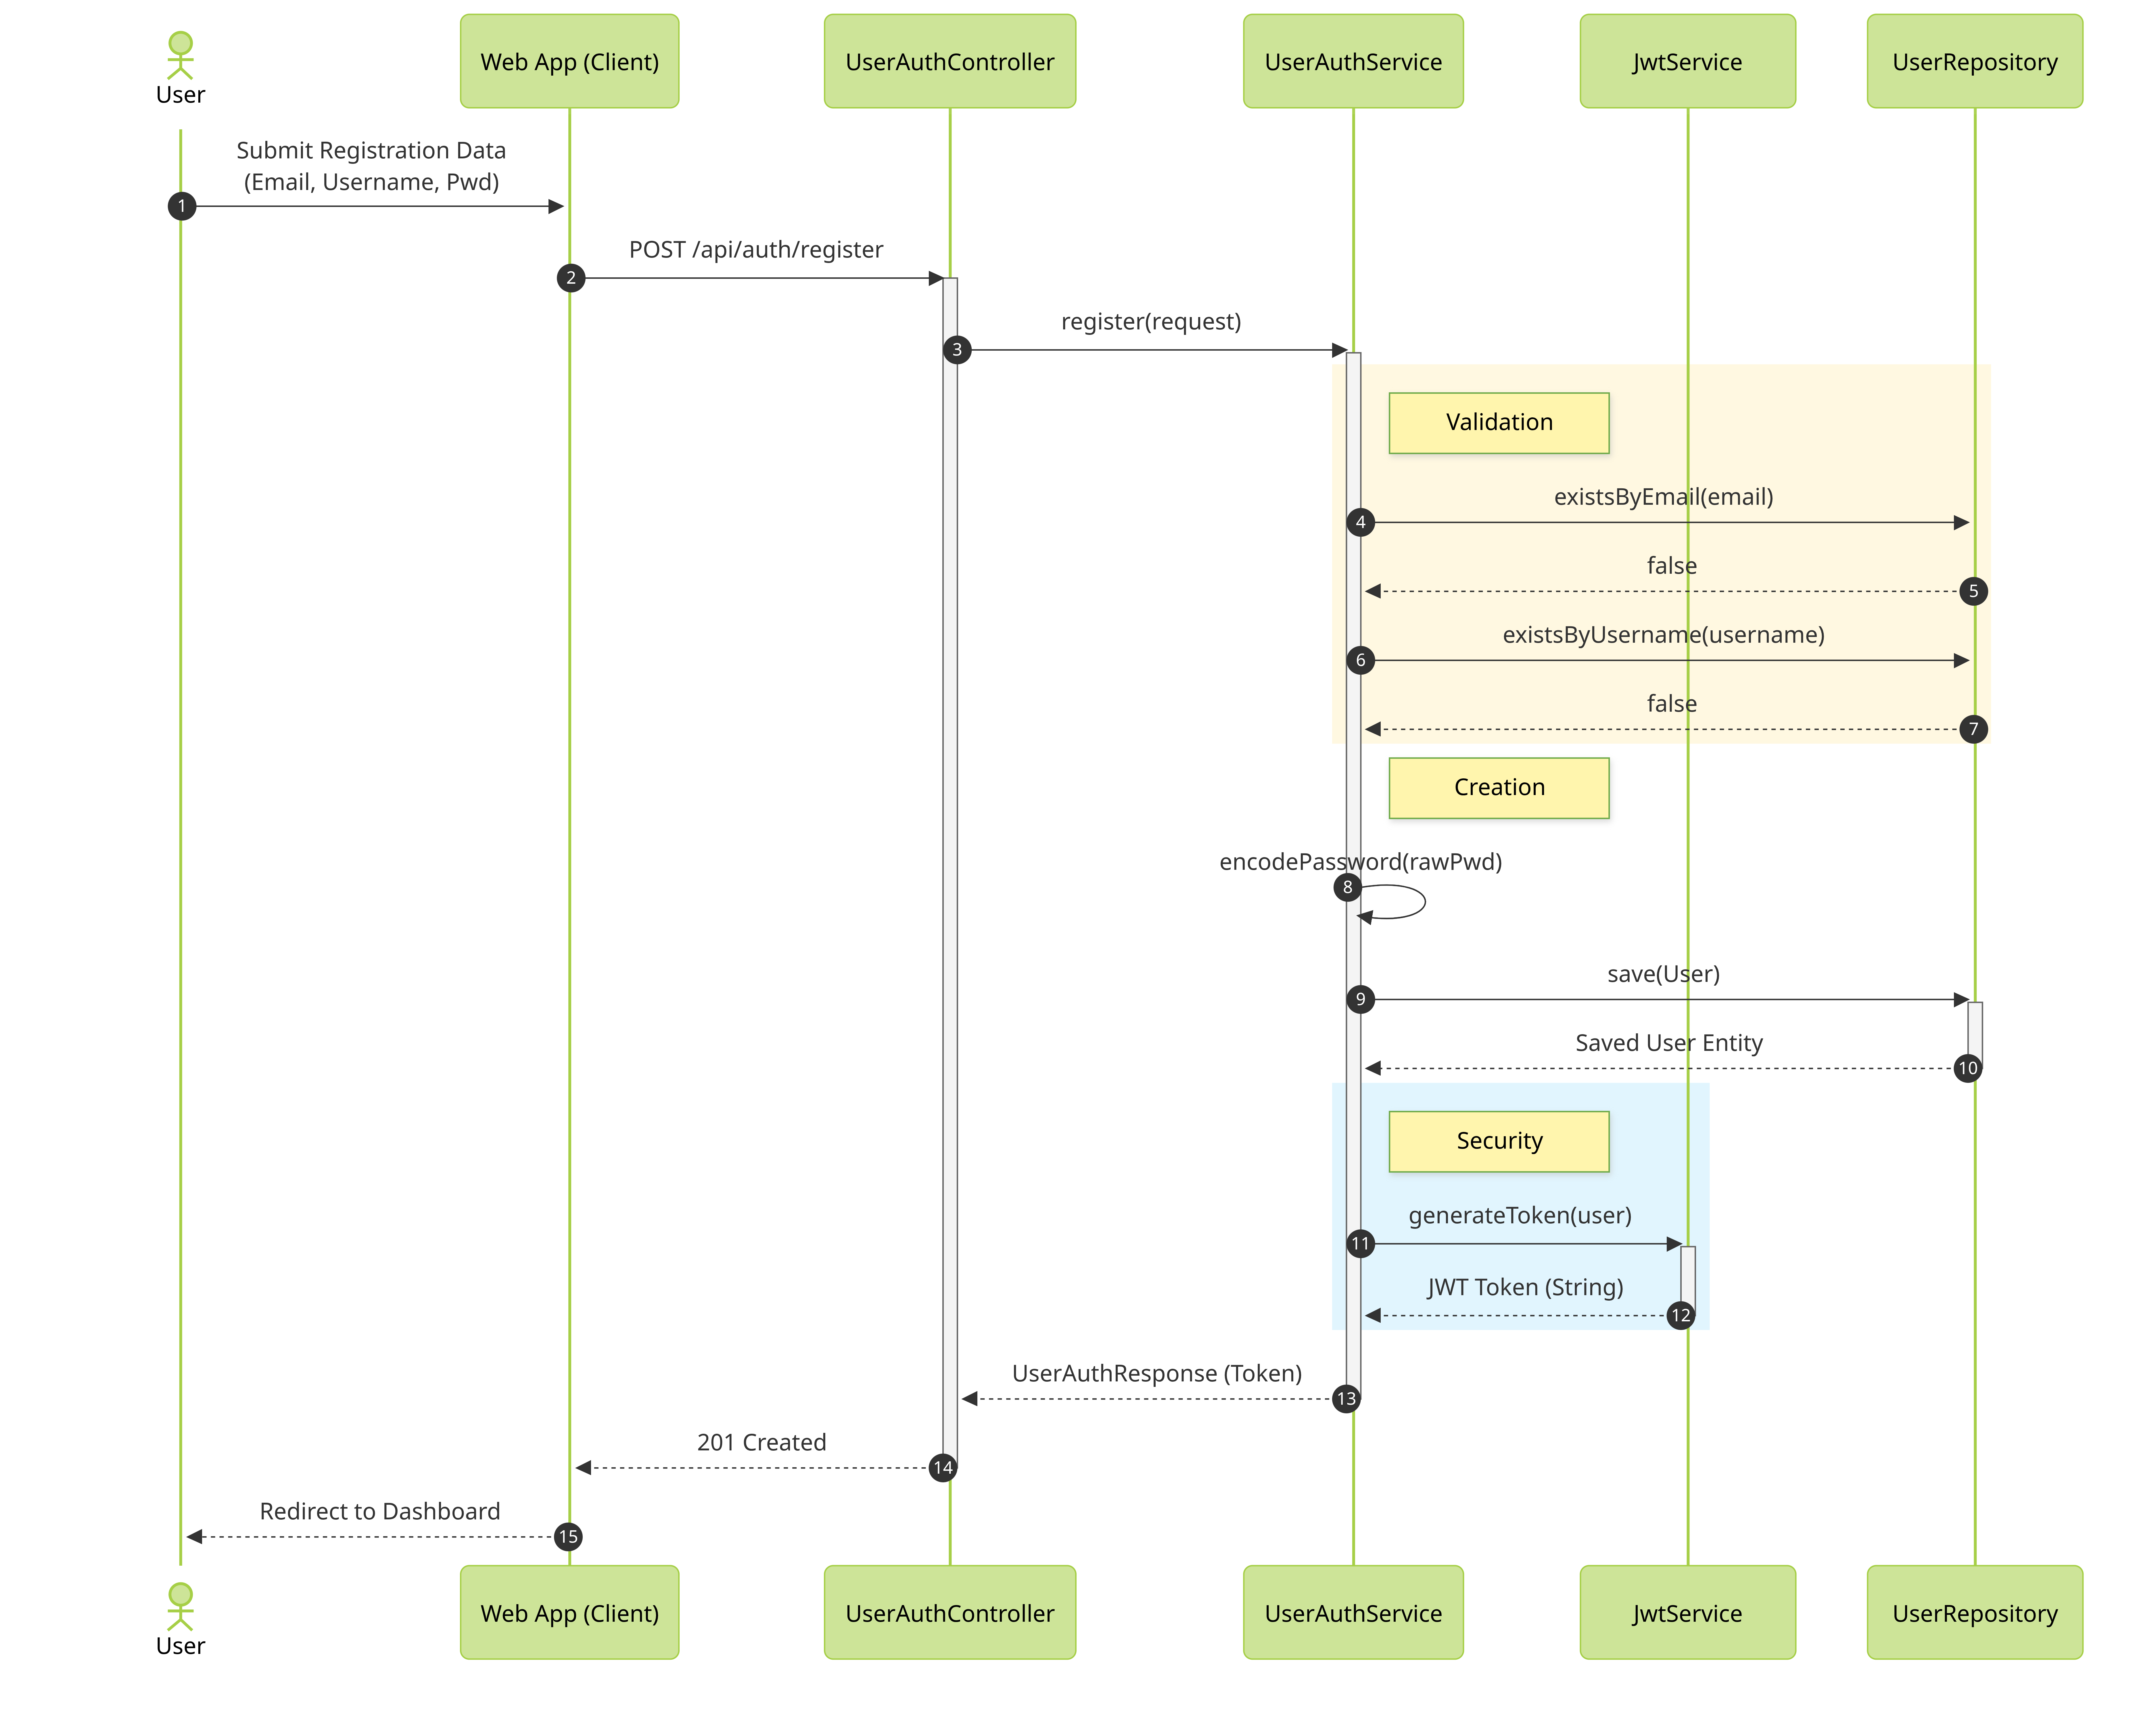
\includegraphics[width=\linewidth, height=\textheight, keepaspectratio]{DD/images/seq_uc6.png}
    \caption{Sequence Diagram - UC6 User Registration}
    \label{fig:seq_uc6}
\end{figure}

\clearpage

\noindent
\textbf{UC7: User Login} \\
The user submits login credentials (email and password). The system verifies the credentials provided; if they are correct, it generates a JWT token and grants access to the dashboard.

\begin{figure}[H]
    \centering
        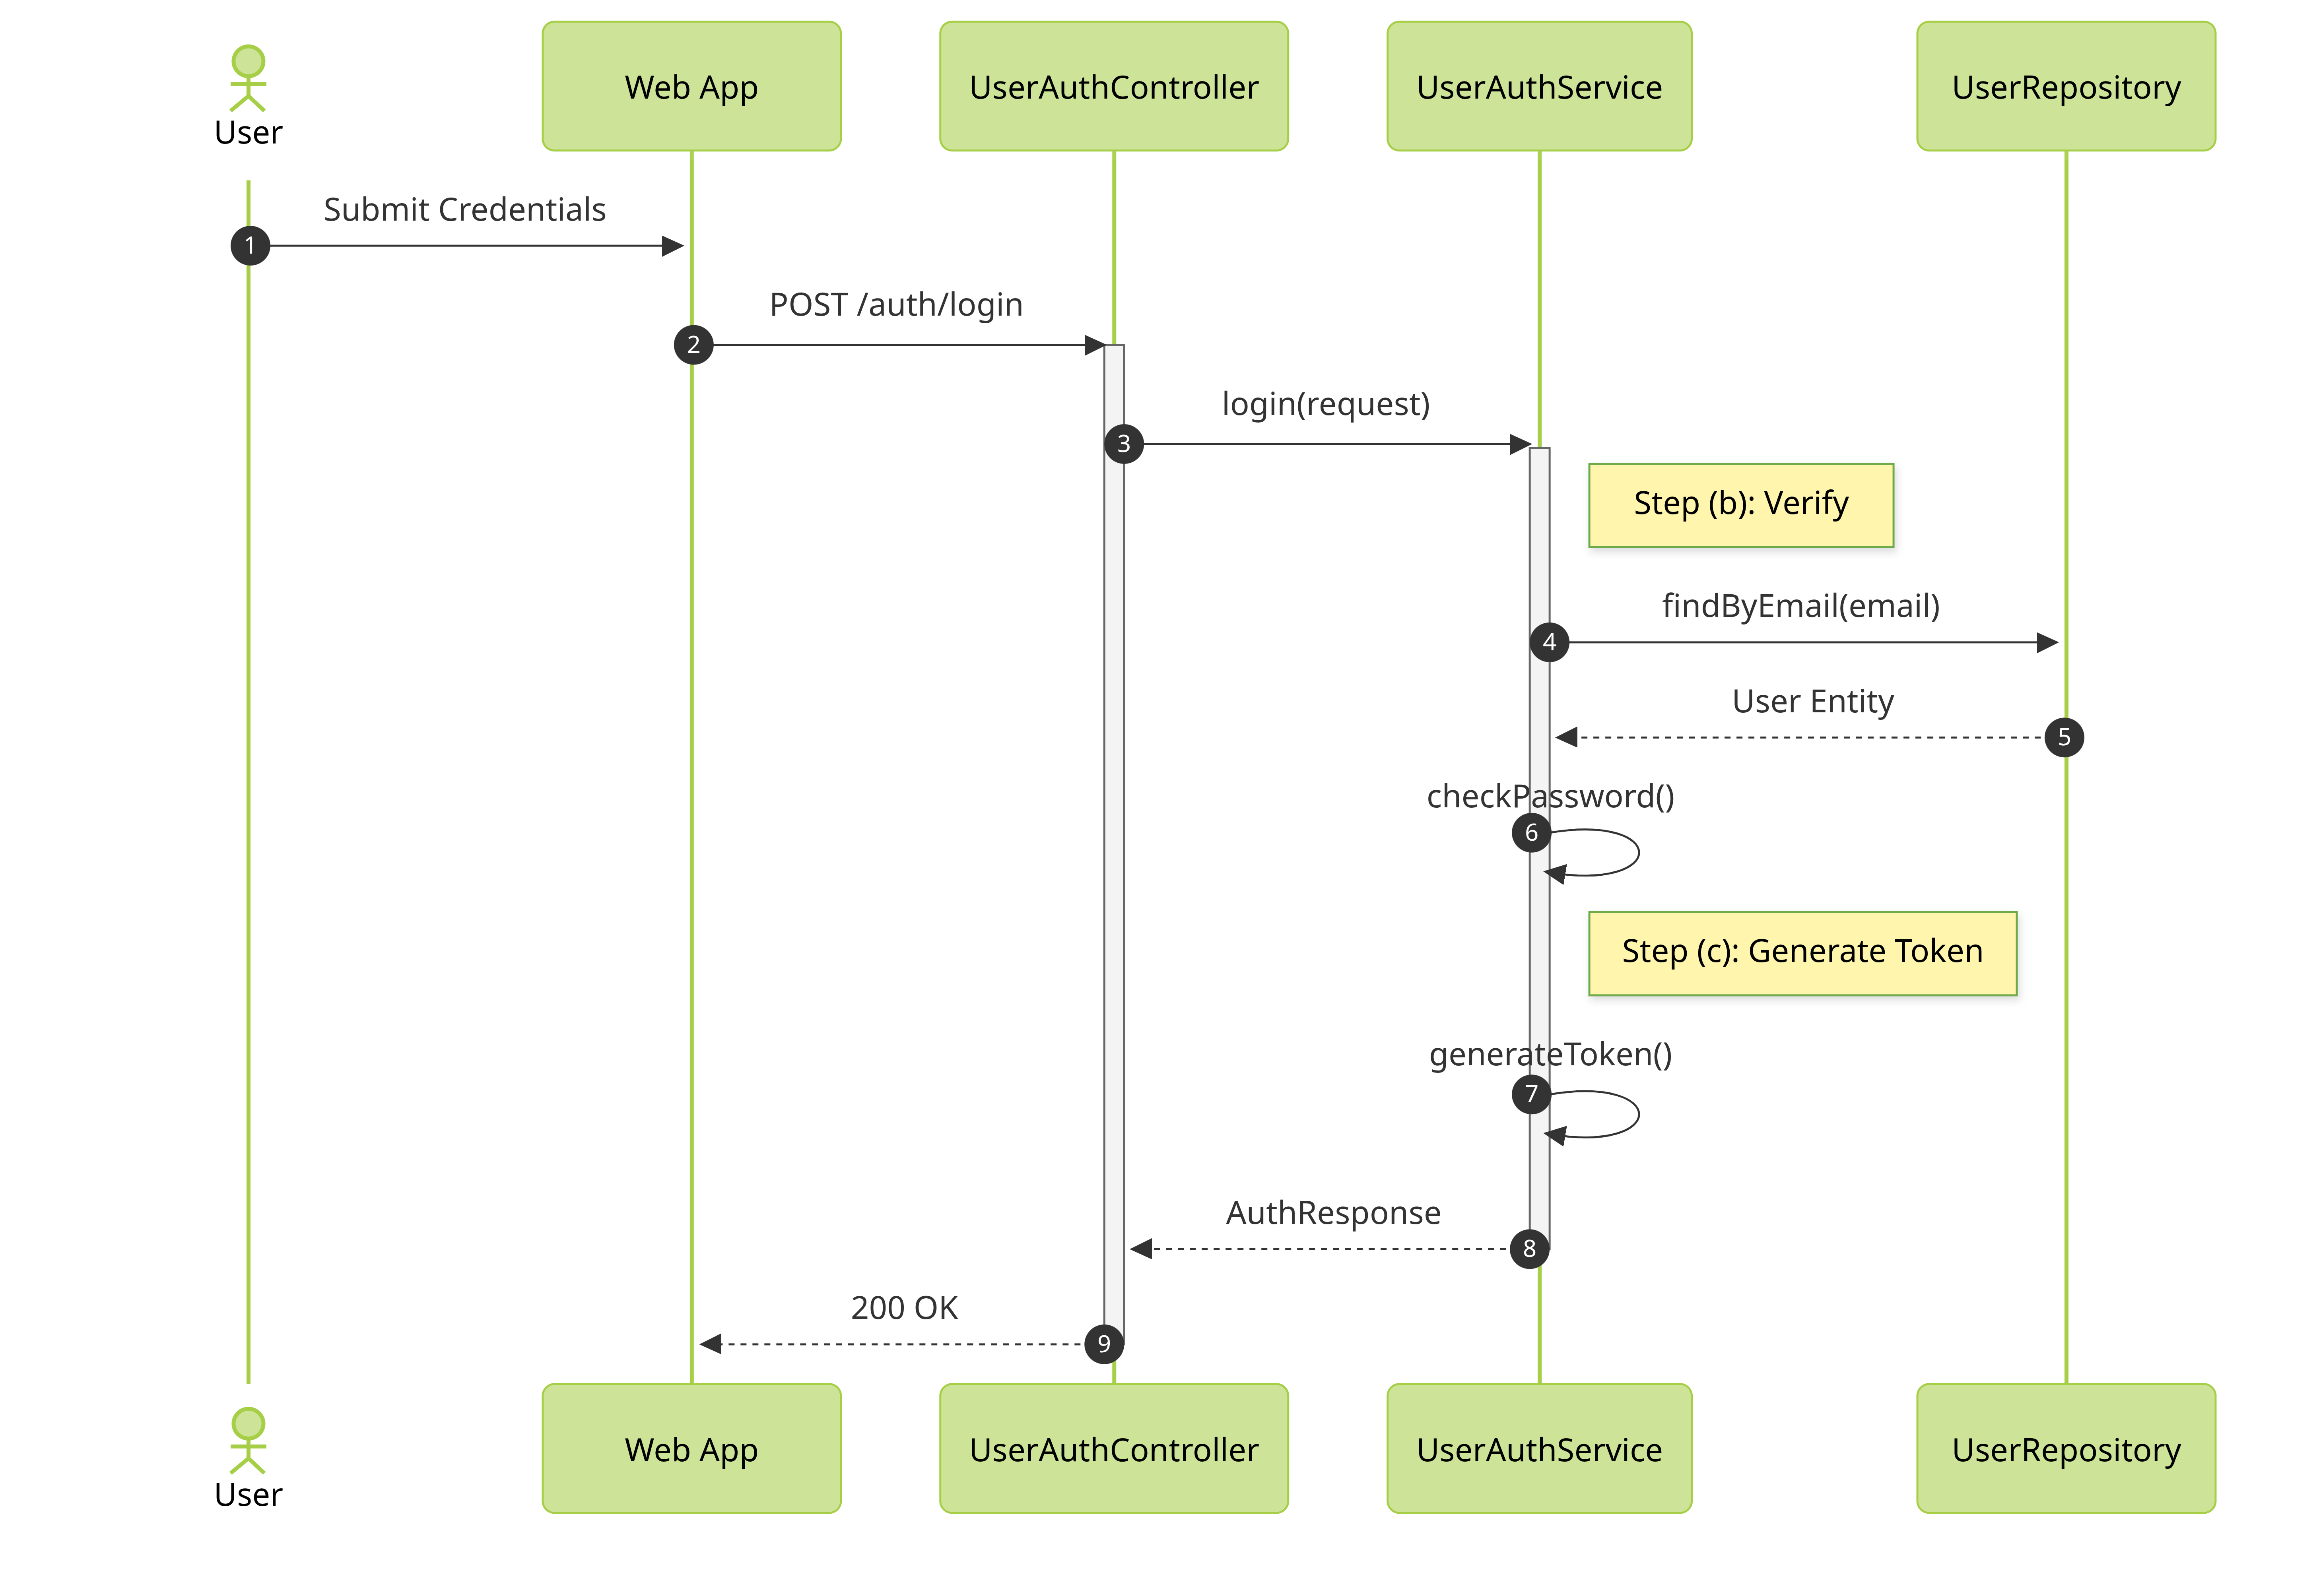
\includegraphics[width=\linewidth, height=\textheight, keepaspectratio]{DD/images/seq_uc7.png}
    \caption{Sequence Diagram - UC7 User Login}
    \label{fig:seq_uc7}
\end{figure}

\clearpage

\noindent
\textbf{UC8: Management of Created Bike Paths} \\
The user manages their created bike paths. The system lists all bike paths created by the user. Depending on the action chosen, the system either updates the bike path metadata (such as visibility or status) or permanently deletes the bike path.

\begin{figure}[H]
    \centering
        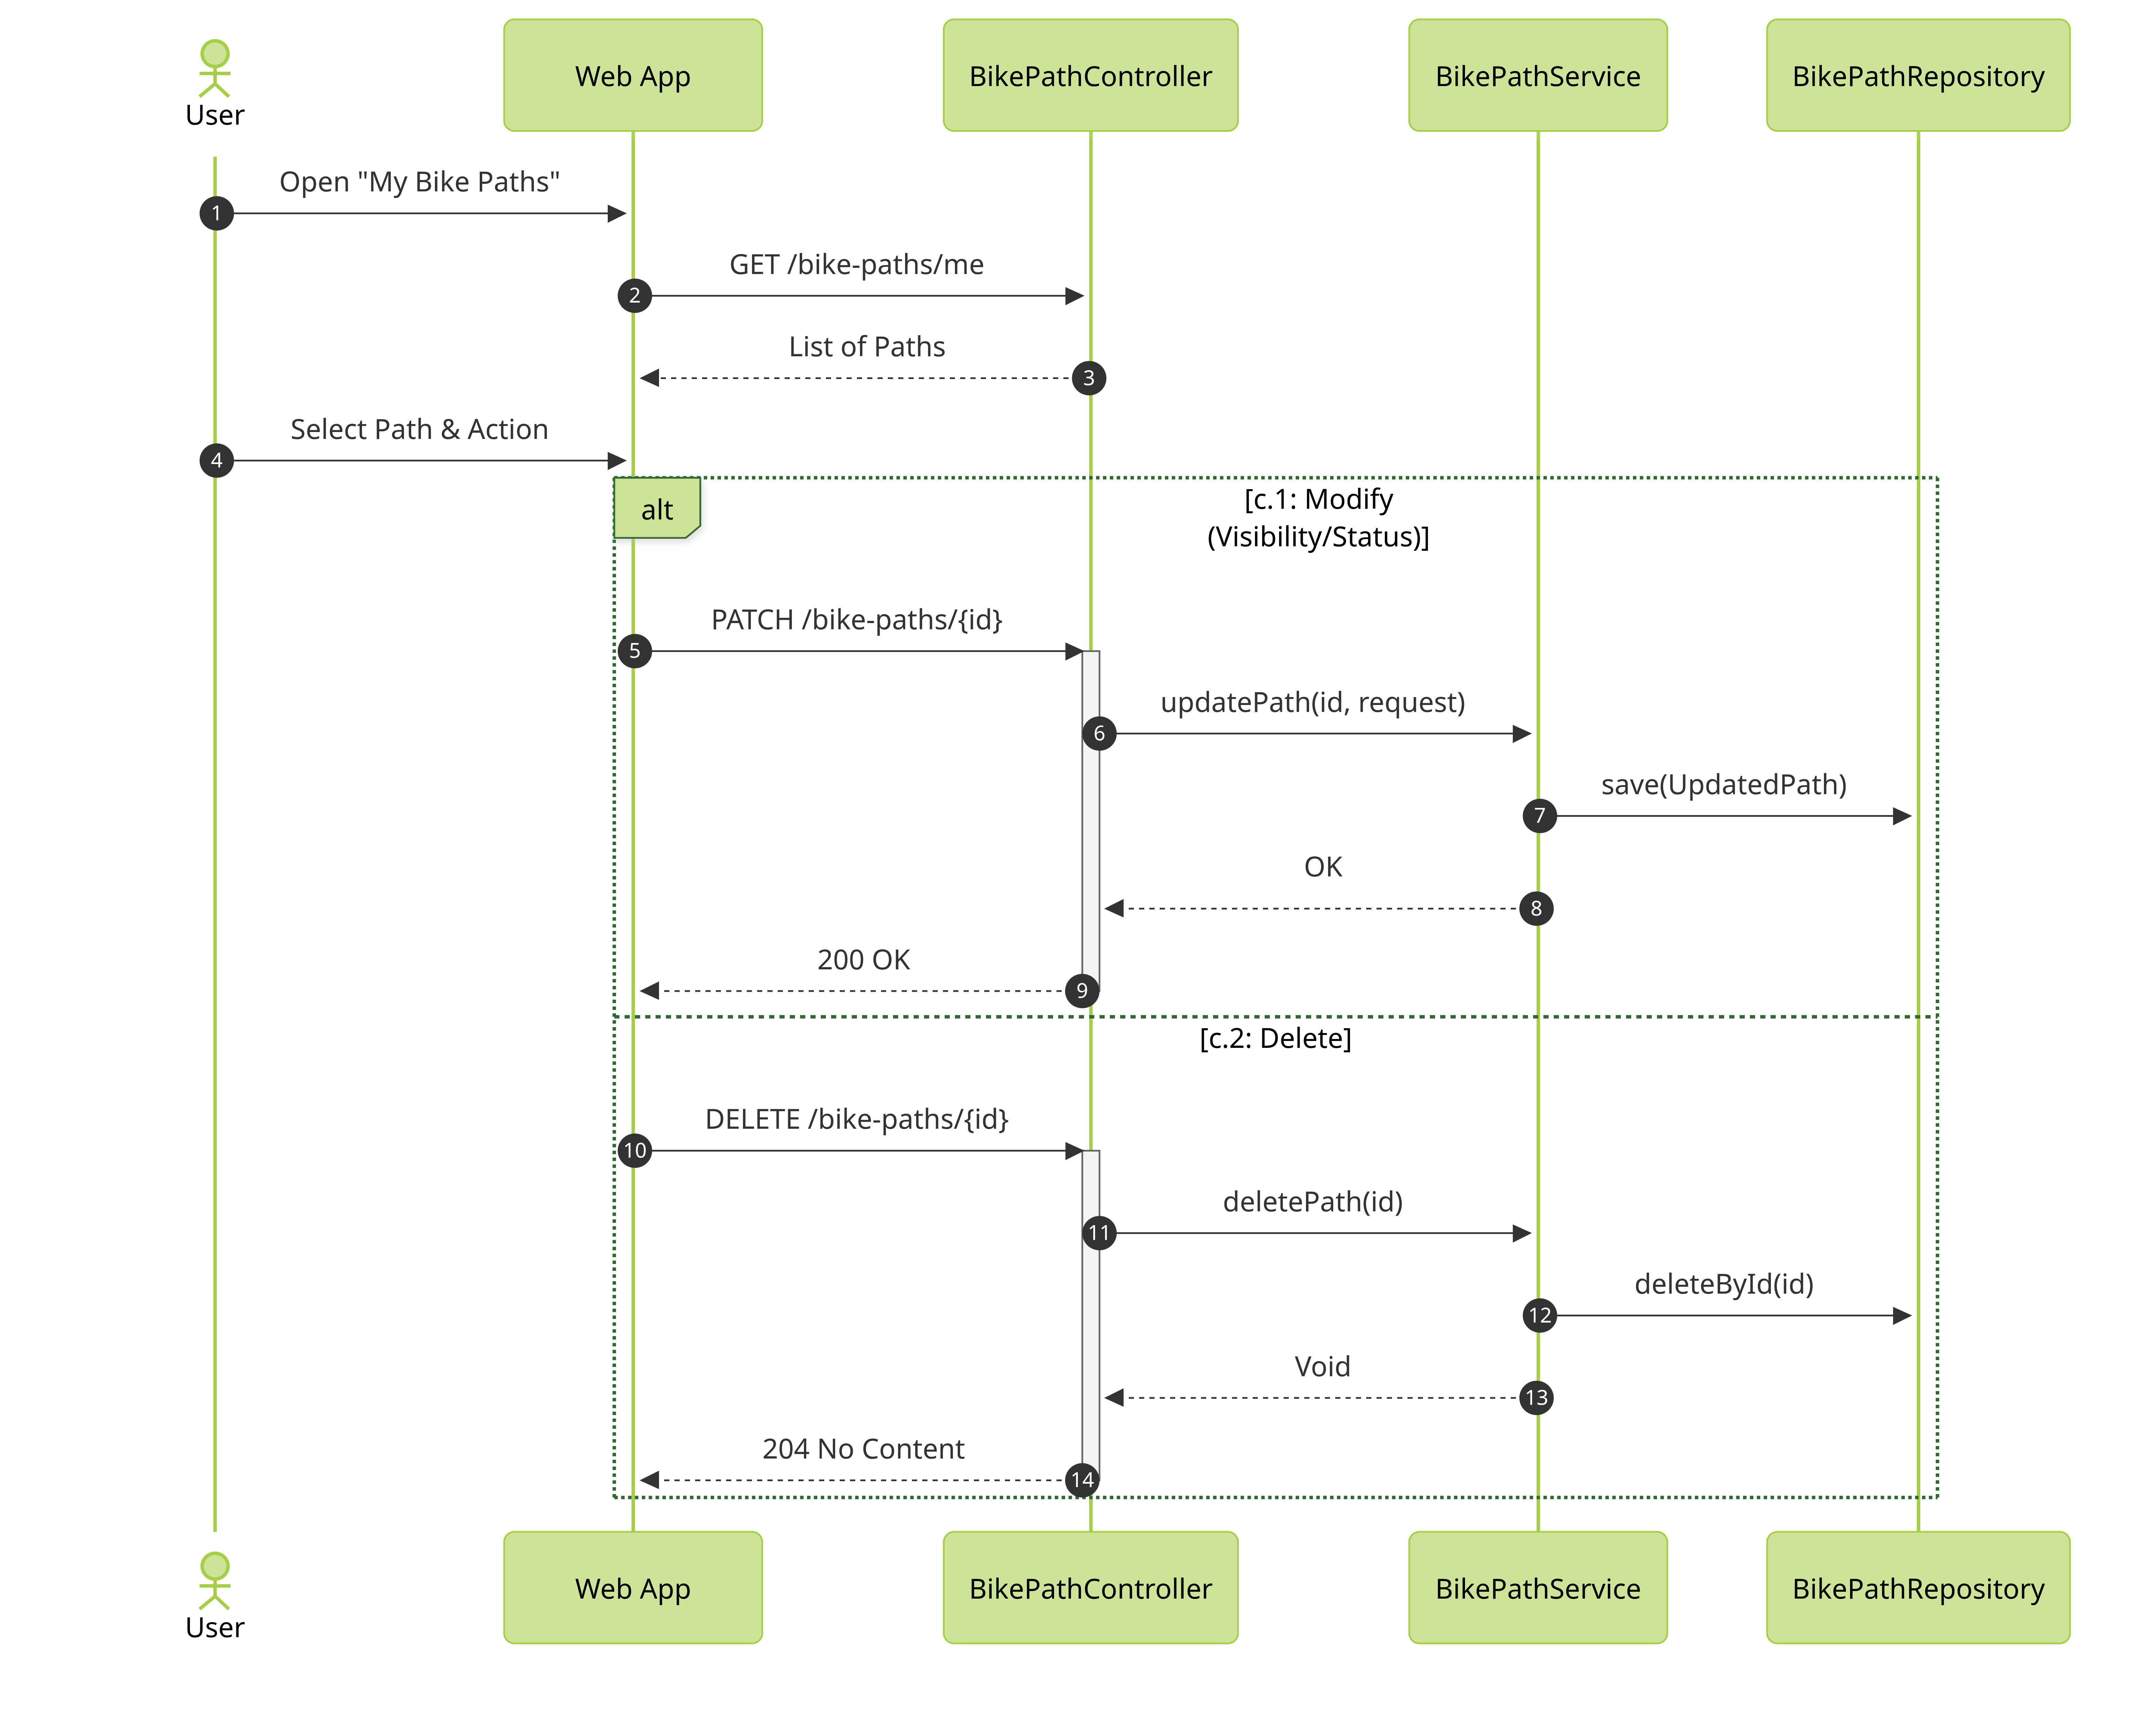
\includegraphics[width=\linewidth, height=\textheight, keepaspectratio]{DD/images/seq_uc8.png}
    \caption{Sequence Diagram - UC8 Management of Created Bike Paths}
    \label{fig:seq_uc8}
\end{figure}

\clearpage

\noindent
\textbf{UC9: Trip History Visualization and Management} \\
The user views their trip history. The system retrieves all trips created by the user, displaying statistics (distance, speed, duration) and associated weather conditions. The user can apply filters to the list or request the deletion of a specific trip, which the system removes from the database.

\begin{figure}[H]
    \centering
        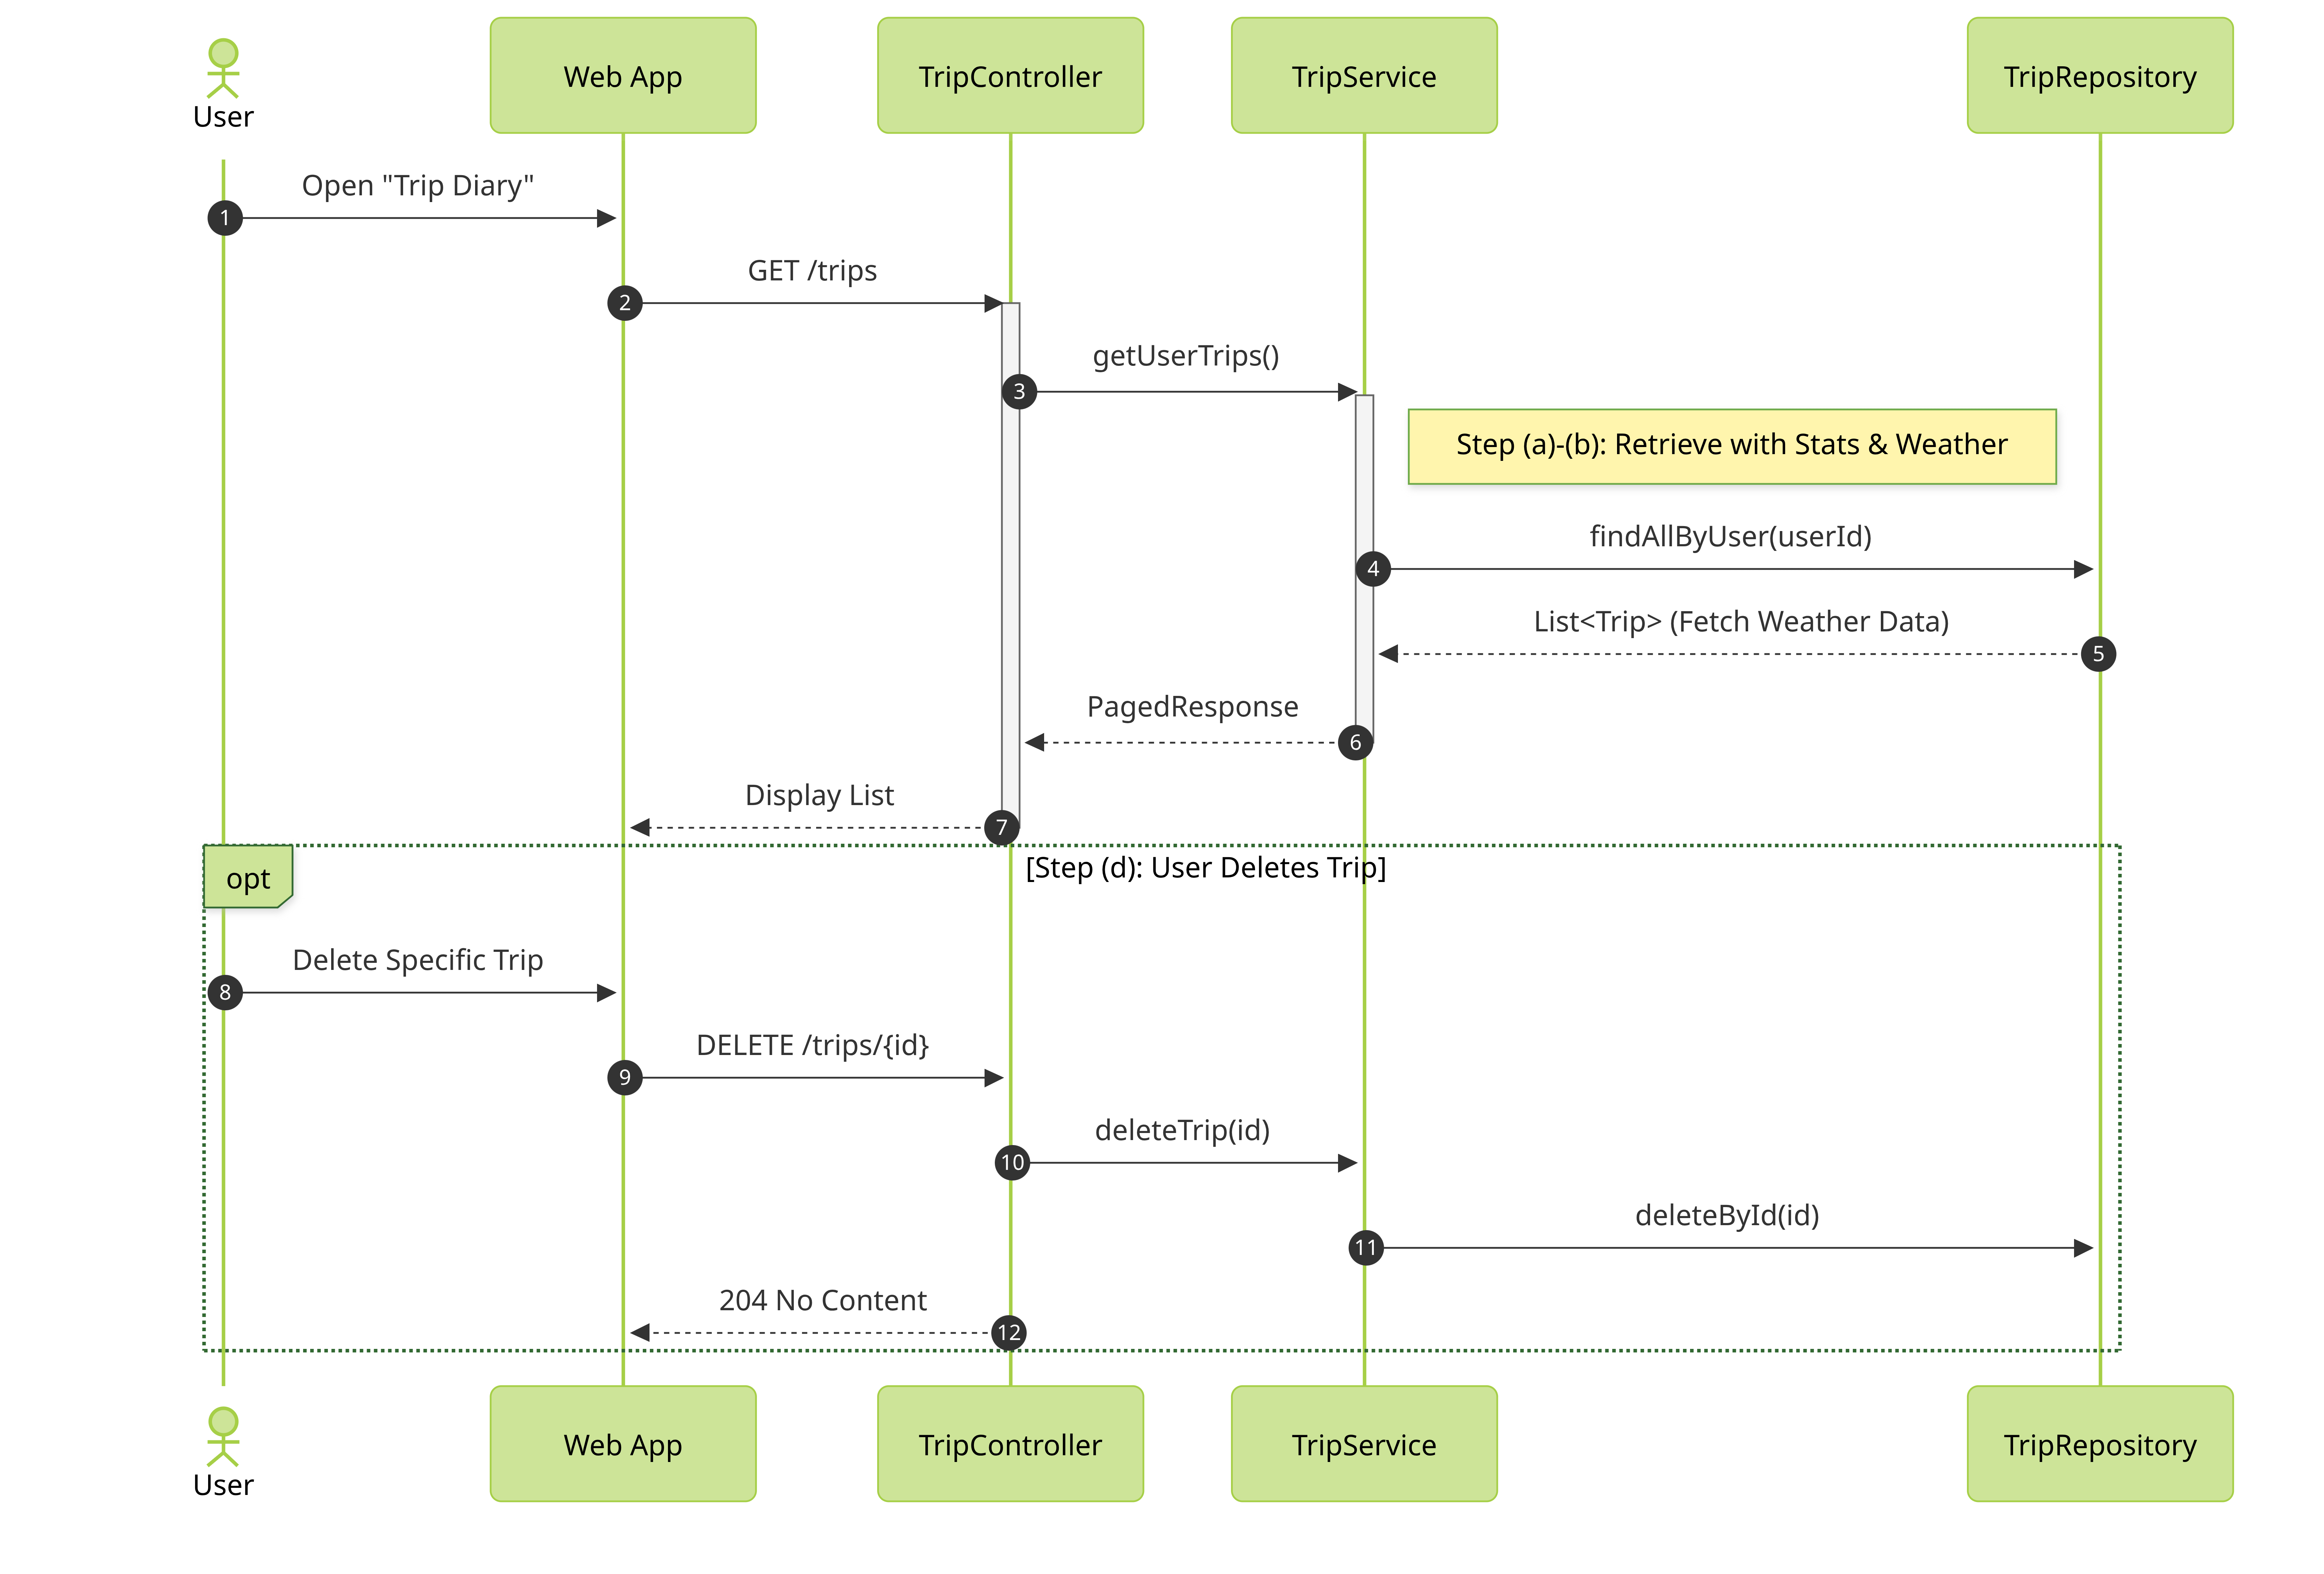
\includegraphics[width=\linewidth, height=\textheight, keepaspectratio]{DD/images/seq_uc9.png}
    \caption{Sequence Diagram - UC9 Trip History Visualization}
    \label{fig:seq_uc9}
\end{figure}

\clearpage

\noindent
\textbf{UC10: User Profile Update} \\
The user modifies their personal data. The system validates the new data; if valid, it updates the user profile and confirms the success of the operation.

\begin{figure}[H]
    \centering
        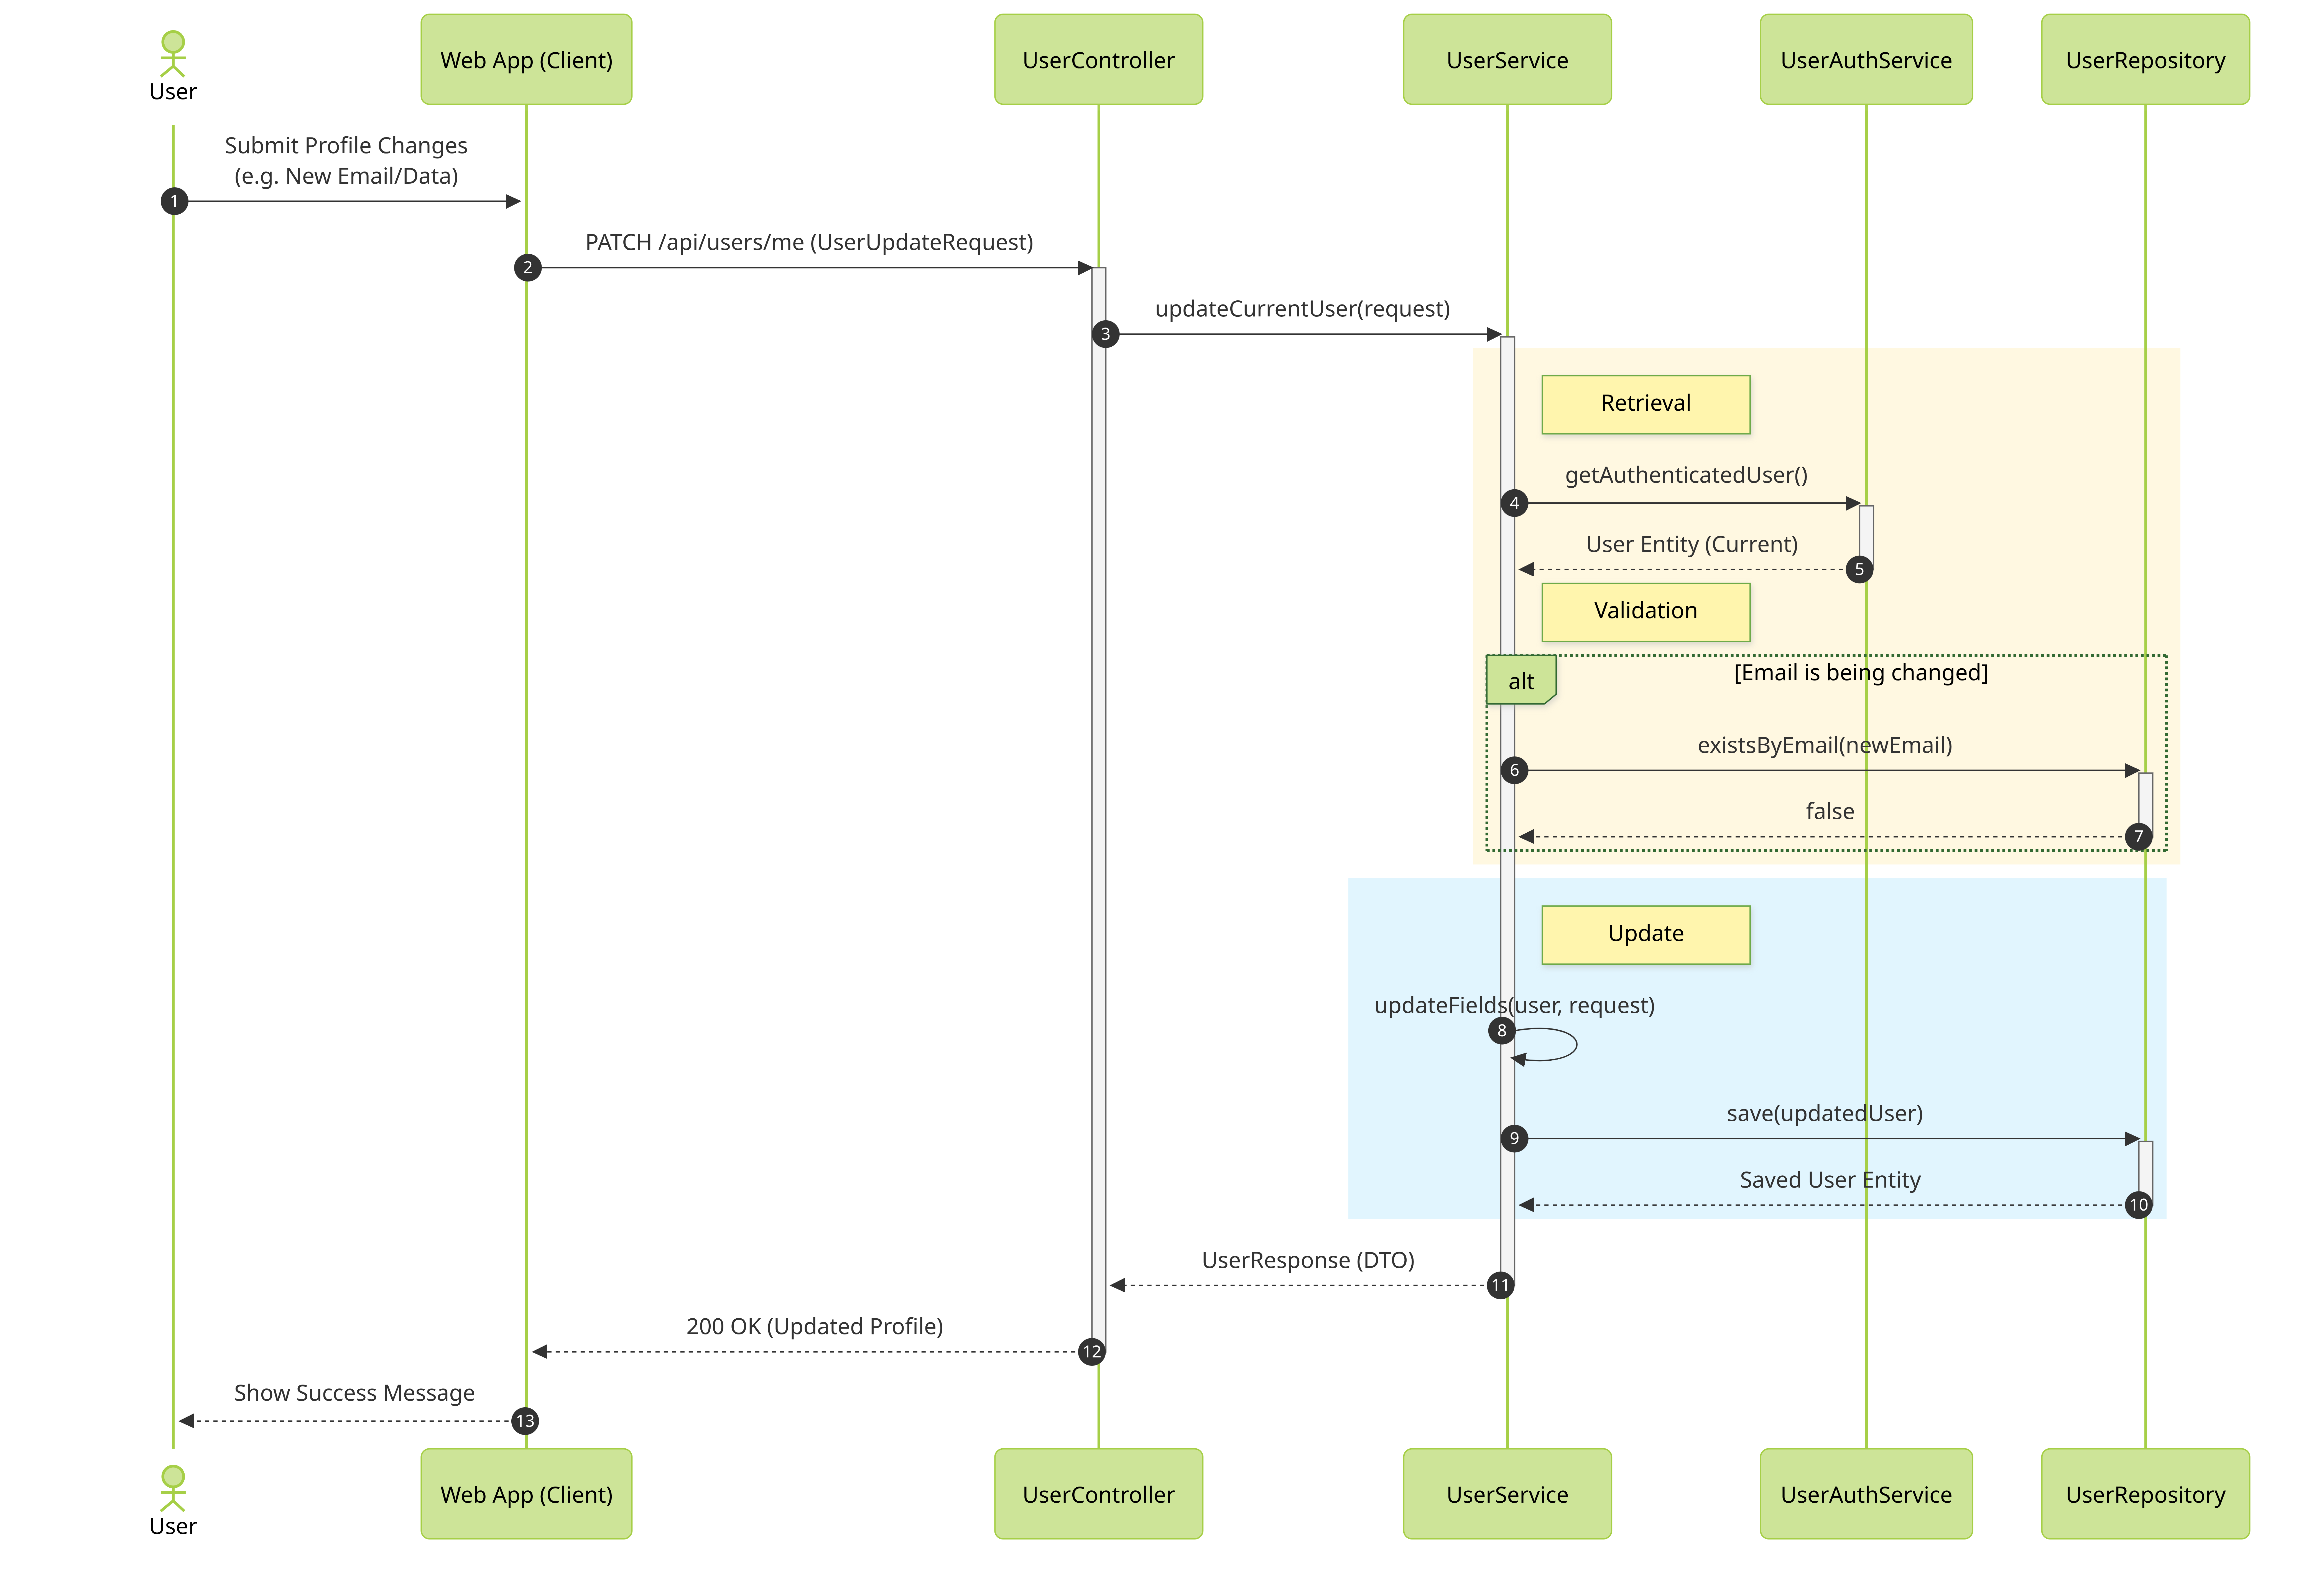
\includegraphics[width=\linewidth, height=\textheight, keepaspectratio]{DD/images/seq_uc10.png}
    \caption{Sequence Diagram - UC10 User Profile Update}
    \label{fig:seq_uc10}
\end{figure}

\clearpage

\subsection{Component Interfaces}
This section shows the interfaces exposed by all the components of the system.

\subsubsection{REST API Interface (Frontend to Backend)}
This interface is exposed by Spring Boot Controllers and consumed by the Client.
\begin{itemize}
    \item \texttt{POST /api/auth/register(UserRegisterRequest)}
    \item \texttt{POST /api/auth/login(UserLoginRequest)}
    \item \texttt{GET /api/users/me}
    \item \texttt{PATCH /api/users/me(UserUpdateRequest)}
    \item \texttt{DELETE /api/users/me}
    \item \texttt{GET /api/trips/\{id\}}
    \item \texttt{GET /api/trips(page, size, sortBy, direction)}
    \item \texttt{POST /api/trips/search(TripSearchRequest, page, size, sortBy, direction)}
    \item \texttt{POST /api/trips/manual(TripManualRecordRequest)}
    \item \texttt{POST /api/trips/automatic(TripAutomaticRecordRequest)}
    \item \texttt{DELETE /api/trips/\{id\}}
    \item \texttt{GET /api/bike-paths/\{id\}}
    \item \texttt{GET /api/bike-paths(page, size, sortBy, direction)}
    \item \texttt{POST /api/bike-paths/search(BikePathSearchRequest, page, size, sortBy, \\ direction)}
    \item \texttt{POST /api/bike-paths/manual(BikePathManualCreateRequest)}
    \item \texttt{POST /api/bike-paths/automatic(BikePathAutomaticCreateRequest)}
    \item \texttt{PATCH /api/bike-paths/\{id\}(BikePathUpdateRequest)}
    \item \texttt{DELETE /api/bike-paths/\{id\}}
    \item \texttt{POST /api/bike-paths/sensor-analysis/validate-anomalies( \\ PreliminaryAnomaliesRequest)}
    \item \texttt{POST /api/finder/bike-paths(BikePathFinderRequest, page, size)}
    \item \texttt{GET /api/mapbox/access-token}
    \item \texttt{POST /api/mapbox/geocode/forward}
    \item \texttt{POST /api/mapbox/geocode/reverse}
    \item \texttt{POST /api/mapbox/cycling-route}
\end{itemize}

\subsubsection{Logic Interfaces}
These interfaces represent the internal business logic invoked by Controllers.

\textbf{UserAuthService Interface}
\begin{itemize}
    \item \texttt{UserAuthResponse register(UserRegisterRequest request)}
    \item \texttt{UserAuthResponse login(UserLoginRequest request)}
    \item \texttt{User getAuthenticatedUser()}
    \item \texttt{User getAuthenticatedUserOrNull()}
\end{itemize}

\textbf{UserService Interface}
\begin{itemize}
    \item \texttt{User updateCurrentUser(UserUpdateRequest request)}
    \item \texttt{void deleteCurrentUser()}
\end{itemize}

\textbf{TripService Interface}
\begin{itemize}
    \item \texttt{Trip recordTripManually(TripManualRecordRequest request)}
    \item \texttt{Trip recordTripAutomatically(TripAutomaticRecordRequest request)}
    \item \texttt{Trip getTripById(Long id)}
    \item \texttt{Page<Trip> getUserTrips(int page, int size, String sortBy, \\ String direction)}
    \item \texttt{Page<Trip> searchTrips(TripSearchRequest request, int page, int size, \\ String sortBy, String direction)}
    \item \texttt{void deleteTrip(Long id)}
\end{itemize}

\textbf{BikePathService Interface}
\begin{itemize}
    \item \texttt{BikePath createBikePathManually(BikePathManualCreateRequest request)}
    \item \texttt{BikePath createBikePathAutomatically(BikePathAutomaticCreateRequest \\ request)}
    \item \texttt{BikePath getBikePathById(Long id)}
    \item \texttt{BikePath updateBikePath(Long id, BikePathUpdateRequest request)}
    \item \texttt{Page<BikePath> getUserBikePaths(int page, int size, String sortBy, \\ String direction)}
    \item \texttt{Page<BikePath> searchBikePaths(BikePathSearchRequest request, int page, \\ int size, String sortBy, String direction)}
    \item \texttt{void deleteBikePath(Long id)}
\end{itemize}

\textbf{ObstacleService Interface}
\begin{itemize}
    \item \texttt{void createAndSaveObstacles(List<ObstacleCreateRequest> requests, \\ BikePath bikePath, List<Coordinate> routeCoordinates, \\ Geometry routeBuffer, User createdBy, OffsetDateTime createdAt)}
    \item \texttt{void updateAndSaveObstacles(BikePath bikePath, \\ List<ObstacleCreateRequest> obstaclesToAdd, List<ObstacleUpdateRequest> \\ obstaclesToUpdate, List<Coordinate> routeCoordinates, \\ Geometry routeBuffer, User updatedBy, OffsetDateTime updatedAt)}
    \item \texttt{BigDecimal calculateObstacleScore(List<Obstacle> obstacles, \\ BigDecimal totalDistance)}
\end{itemize}

\textbf{BikePathFinderService Interface}
\begin{itemize}
    \item \texttt{Page<BikePath> findBikePaths(BikePathFinderRequest request, int page, \\ int size)}
\end{itemize}

\textbf{SensorAnalysisService Interface}
\begin{itemize}
    \item \texttt{List<EnrichedAnomaly> validateAndEnrichAnomalies(List<PreliminaryAnomaly> \\ preliminaryAnomalies)}
\end{itemize}

\subsubsection{External Services Interfaces}
These interfaces are used by internal adapters to communicate with third-party systems.

\textbf{MapboxService Interface}
\begin{itemize}
    \item \texttt{GeocodeResult geocodeAddress(String address)}
    \item \texttt{List<GeocodeResult> geocodeAddresses(List<String> addresses)}
    \item \texttt{GeocodeResult geocodeCoordinate(Coordinate coordinate)}
    \item \texttt{CyclingRouteResult calculateCyclingRoute(List<Coordinate> waypoints)}
\end{itemize}

\textbf{OpenMeteoService Interface}
\begin{itemize}
    \item \texttt{MeteorologicalData getWeatherData(Double latitude, Double longitude, \\ OffsetDateTime startTime, Trip trip)}
    \item \texttt{MeteorologicalDataResult fetchWeatherData(Double latitude, \\ Double longitude, OffsetDateTime startTime)}
\end{itemize}

\subsubsection{DBMS Interfaces (Repository Layer)}
Spring Data JPA repositories for persistence operations with PostgreSQL+PostGIS database. \\
Route geometries stored as GEOMETRY(LineString, 4326) and obstacle locations as GEOMETRY(Point, 4326). \\
Spatial operations performed using PostGIS native functions with GiST indexes for performance.

\textbf{UserRepository}
\begin{itemize}
    \item \texttt{Optional<User> findByEmail(String email)}
    \item \texttt{boolean existsByUsername(String username)}
    \item \texttt{boolean existsByEmail(String email)}
    \item Standard JPA CRUD operations (save, findById, delete)
\end{itemize}

\textbf{TripRepository}
\begin{itemize}
    \item \texttt{Page<Trip> findPageByRecordedByIdWithWeather(Long userId, \\ Pageable pageable)}
    \item Native spatial queries using PostGIS functions (ST\_Length, ST\_AsGeoJSON) for route geometry operations
    \item Standard JPA CRUD operations
\end{itemize}

\textbf{BikePathRepository}
\begin{itemize}
    \item \texttt{Page<BikePath> findPageByCreatedById(Long userId, Pageable pageable)}
    \item \texttt{List<BikePath> findPublishedWithinRadius(Point origin, Point destination, \\ double radiusKm)}
    \item Native spatial queries using ST\_DWithin for geographic proximity search on origin/destination points
    \item Standard JPA CRUD operations and JpaSpecificationExecutor for dynamic filtering
\end{itemize}

\textbf{ObstacleRepository}
\begin{itemize}
    \item \texttt{List<Obstacle> findAllByBikePathIdOrderByPositionOnPathAsc( \\ Long bikePathId)}
    \item Spatial validation queries using ST\_Buffer and ST\_Within to verify obstacle proximity to route geometry
    \item Standard JPA CRUD operations for obstacle persistence
\end{itemize}

\textbf{MeteorologicalDataRepository}
\begin{itemize}
    \item Standard JPA CRUD operations only
\end{itemize}

\textbf{Spatial Operations:}
PostGIS functions used include ST\_DWithin (distance queries), ST\_Buffer (proximity zones), 
ST\_Within (containment), ST\_Distance (precise distance calculation), ST\_Length (route distance), 
and ST\_AsGeoJSON (geometry serialization). GiST spatial indexes on geometry columns ensure efficient query performance.


\subsection{Selected Architectural Styles and Patterns}
The architecture of the BBP system integrates various well-known patterns of software engineering. The combination of these solutions has been designed to ensure a high degree of modularity and to simplify code maintenance.

\subsubsection{Client-Server Architecture (RESTful)}
The system is based on a client-server architecture that completely decouples the presentation layer from the business logic and data. The frontend consists of a web application built in Vue.js and a native mobile application developed with Flutter. Both the web and mobile clients, along with the backend based on Spring Boot, operate as separate entities that communicate exclusively through RESTful API interfaces. The server exposes stateless HTTP endpoints that return data in standard JSON format, consumed by the clients via asynchronous libraries.

\subsubsection{Layered Architecture (Three-Layer)}
Internally, the backend is structured according to a layered architecture pattern, imposing a strict segregation of responsibilities. The flow of a request passes through three distinct layers:
\begin{enumerate}
    \item \textbf{Controller Layer}: Manages the HTTP interface, validating inputs and serializing responses.
    \item \textbf{Service Layer}: Encapsulates the core logic of the application.
    \item \textbf{Repository Layer}: Abstracts access to persistent data.
\end{enumerate}
This layering reduces coupling between components and facilitates the writing of isolated unit tests, allowing business logic to be tested independently of the other parts.

\subsubsection{Dependency Injection \& Inversion of Control}
The Spring Boot framework is used to implement the principle of Inversion of Control through Dependency Injection. Instead of manually instantiating dependencies, components delegate this responsibility to the Spring container, which automatically injects the necessary instances when the application starts. This approach, managed through annotations such as @Autowired or @RequiredArgsConstructor, makes the code more testable, allowing for the easy injection of mock objects during testing.

\subsubsection{Data Transfer Object Pattern}
To decouple the internal domain model from the contract exposed externally via APIs, the system adopts the Data Transfer Object pattern. Data do not travel across the network as database entities, but are encapsulated in dedicated DTO objects. The use of specific mappers for Entity-DTO conversion allows sensitive attributes to be hidden, data from different sources to be aggregated, and public APIs to remain stable even when changes are made to the database schema.

\subsubsection{Adapter Pattern}
Integration with third-party services, such as Mapbox for mapping and Open-Meteo for weather data, is managed through the Adapter Pattern. Specific classes such as MapboxService act as adapters, exposing high-level, semantically rich methods to the domain while hiding the complexity of raw HTTP calls and parsing external responses. This isolation protects the business logic from any changes in external providers' APIs.

\subsubsection{Repository Pattern}
Data access is abstracted via the Repository Pattern, implemented with Spring Data JPA. Dedicated interfaces provide a collection-like view of domain objects, hiding the details of the underlying SQL queries. In addition to standardizing the creation, reading, updating and deletion operations, this pattern allows for the declarative definition of complex queries, including PostGIS spatial operations.

\subsection{Other Design Decisions}
In addition to structural architectural patterns, specific technical decisions were made to meet the security and data management requirements.

\subsubsection{Spatial data handling: PostGIS}
Given the geospatial nature of the project, the system avoids representing coordinates as simple numerical pairs in favor of native geometric types. The adoption of PostgreSQL with the PostGIS extension allows the computational load of spatial operations to be delegated to the DBMS. Complex queries, such as searching for paths within a bounding box or calculating intersections, are performed natively and efficiently directly at the database level.

\subsubsection{Stateless Authentication: JSON Web Token}
To maximize scalability, the system uses a stateless authentication mechanism based on JSON Web Token standards, eliminating the need to manage server-side sessions and session cookies. Each authenticated request carries a signed token that identifies the user, allowing the backend to scale horizontally without having to replicate the session state across nodes. Furthermore, this approach facilitates cross-platform integration, allowing web and mobile clients to handle authentication in a uniform manner.